\documentclass{article}
\usepackage[a4paper, total={7in, 10in}]{geometry}
\usepackage{fontspec} 
\usepackage{xeCJK} 
\setCJKmainfont{標楷體}
\setmainfont{Times New Roman}
\XeTeXlinebreaklocale “zh” 
\XeTeXlinebreakskip = 0pt plus 1pt
\usepackage{graphicx}
\usepackage{float}
\usepackage{xcolor}
\usepackage[linesnumbered,ruled,vlined]{algorithm2e}
\usepackage{mathtools}
\usepackage{amsmath} 
\usepackage{subfigure}  




\newcommand\mycommfont[1]{\footnotesize\ttfamily\textcolor{blue}{#1}}
\SetCommentSty{mycommfont}

\SetKwInput{KwInput}{Input}                % Set the Input
\SetKwInput{KwOutput}{Output}              % set the Output

\title{Self-Driving Cars}
\author{309611087 洪得瑜}
\date{2022 10/20} 

\begin{document}
\maketitle
\section{Part 1 Motion Dataset}
Matplotlib 視覺化場景:
\begin{itemize}
	\item 歷史軌跡: 綠色
	\item 未來軌跡: 紅色 
	\item 道路中線: "- -" 白色
	\item 道路邊線: 灰色
	\item 斑馬線: 紫色
	\item 周圍動態軌跡: 藍色
\end{itemize}
\begin{figure}[H]
	\centering
	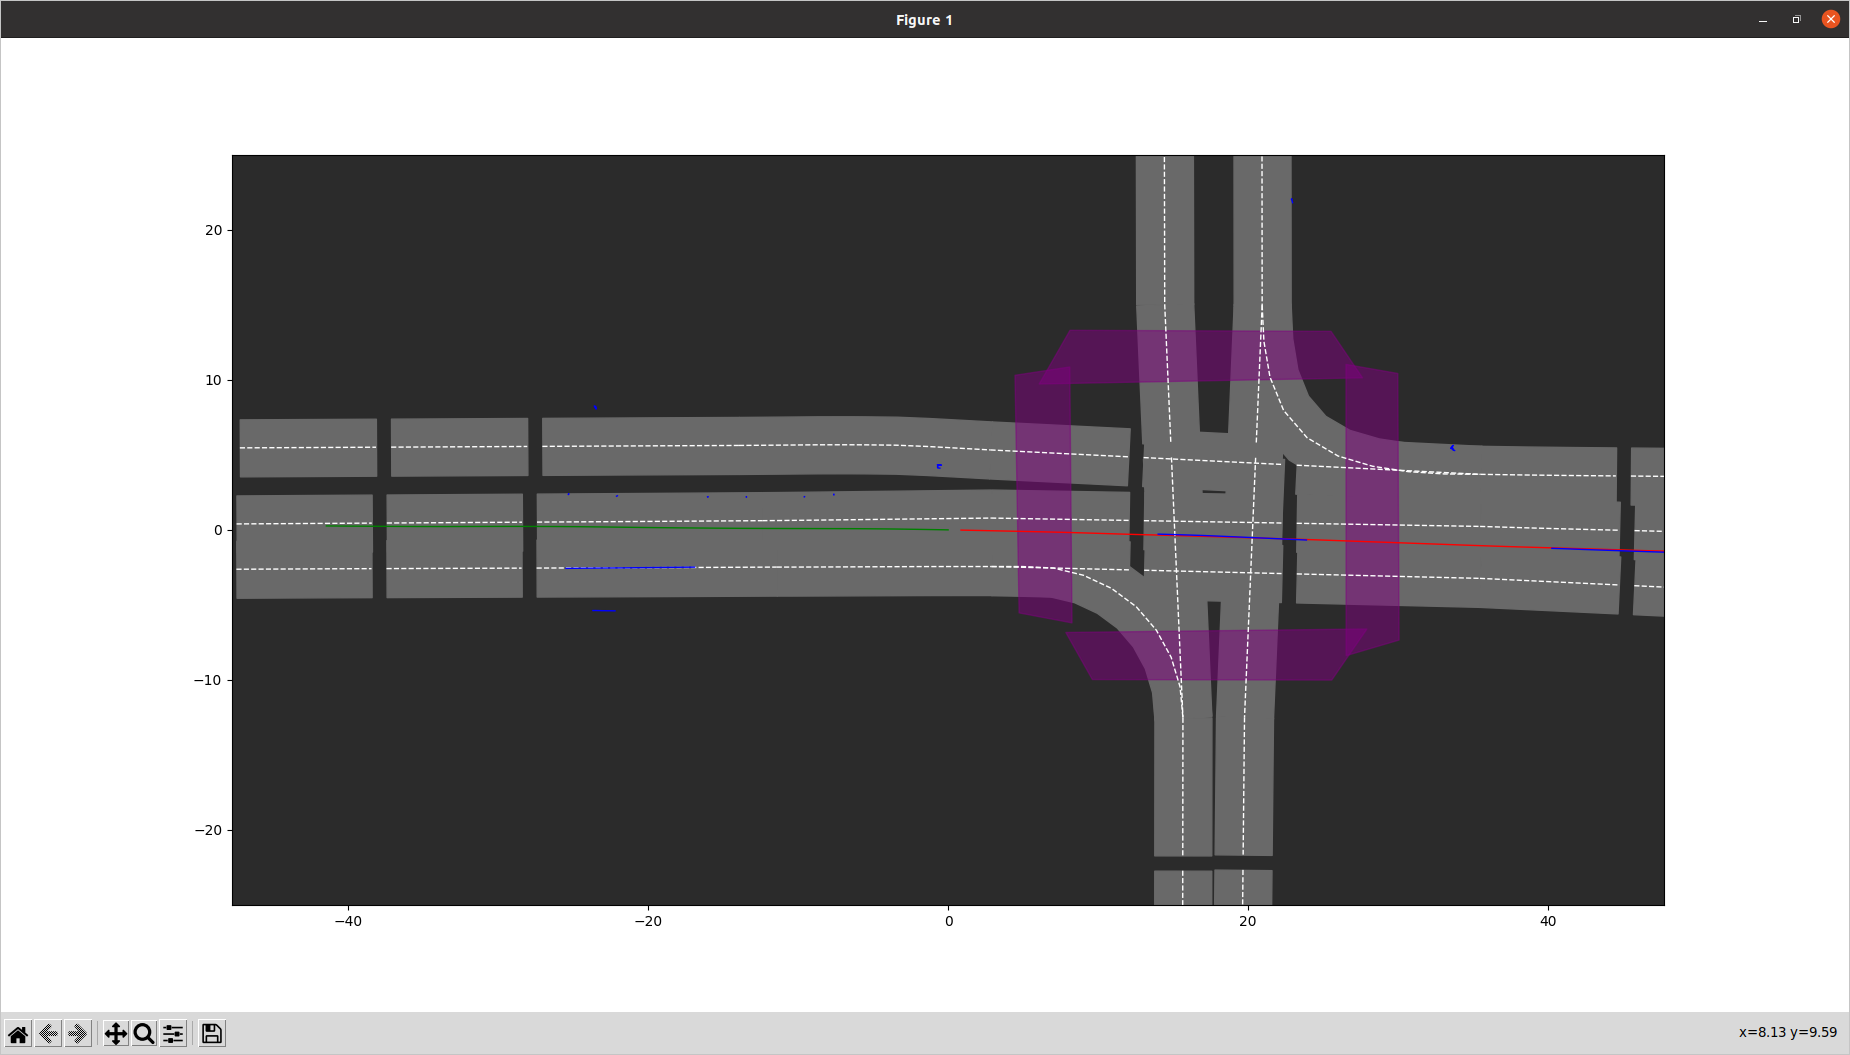
\includegraphics[scale=0.3]{./lane.png}
	\caption{Dataset 場景圖}
\end{figure}

\subsection{Code}
\begin{figure}[H]
	\centering
	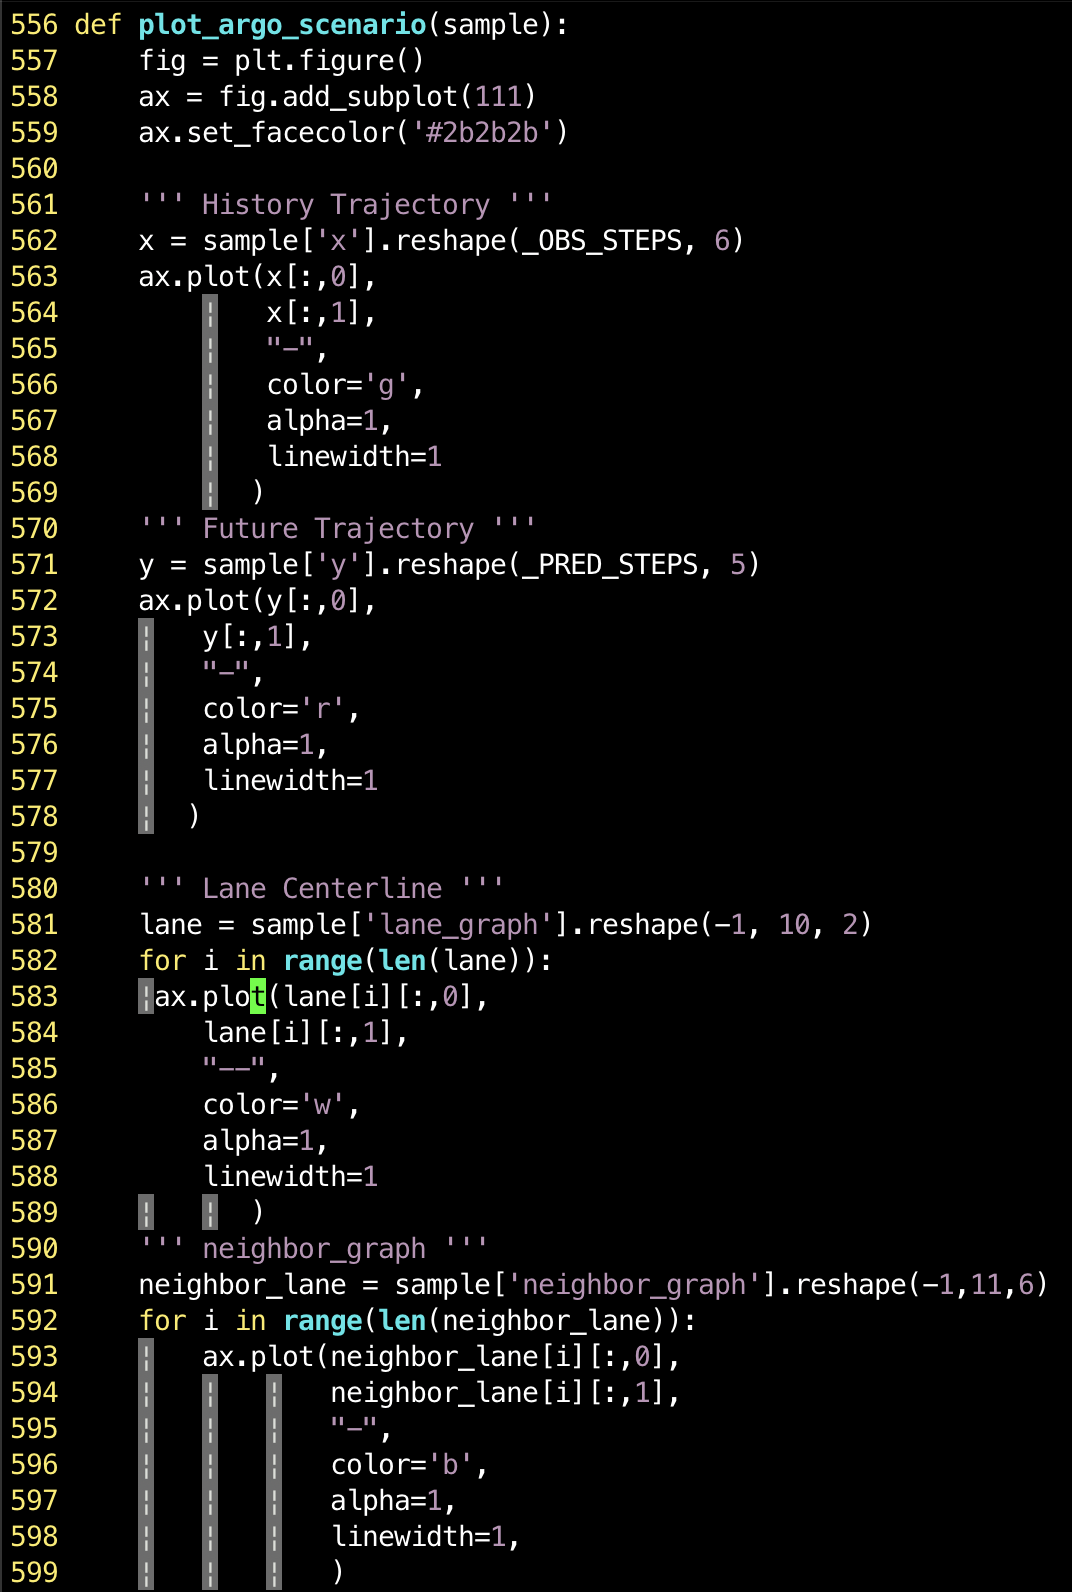
\includegraphics[scale=0.5]{./part1_1.png}
\end{figure}

\begin{figure}[H]
	\centering
	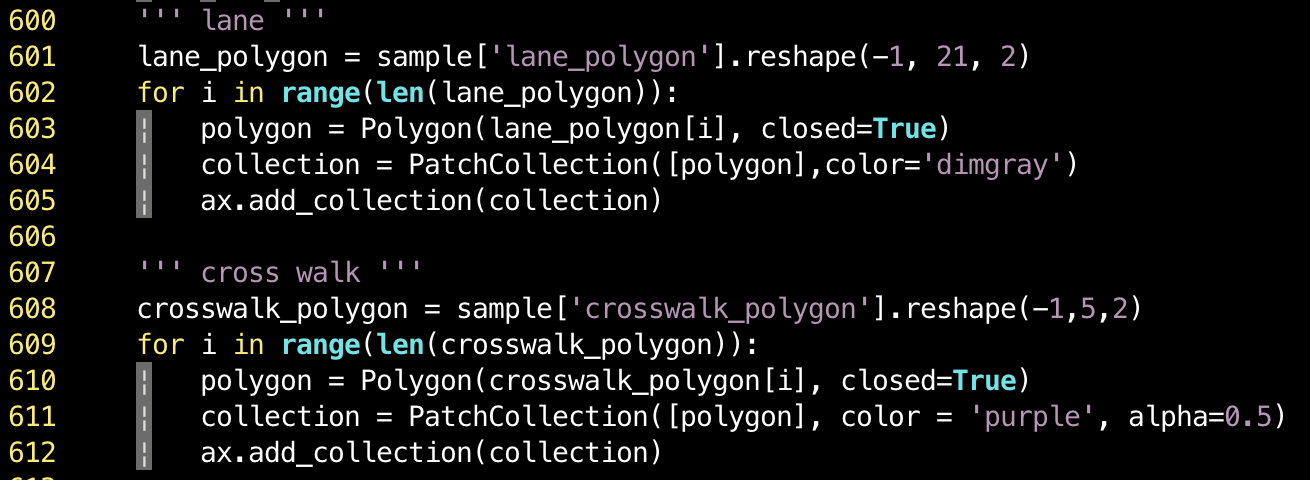
\includegraphics[scale=0.5]{./part1_2.png}
\end{figure}

\section{Part 2}

Model Design:
Model中Baseline參考文獻[1][2]設計,建立高精地圖特徵MapNet[1]使用向量化地圖建構車道圖,而文獻[1]中以LaneGCN方法輸出地圖特徵,結合周遭動態特徵及車道特徵進行動態預測,而在本次車道與周圍關係以文獻[2]VectorNet方法將高經地圖特徵與車道及周圍動態融合,VectorNet將同一元素以向量組成行成一條poyline將多個polylines行成Subgraph,將所有軌跡和地圖特徵全局分析。
\begin{figure}[H]
	\centering
	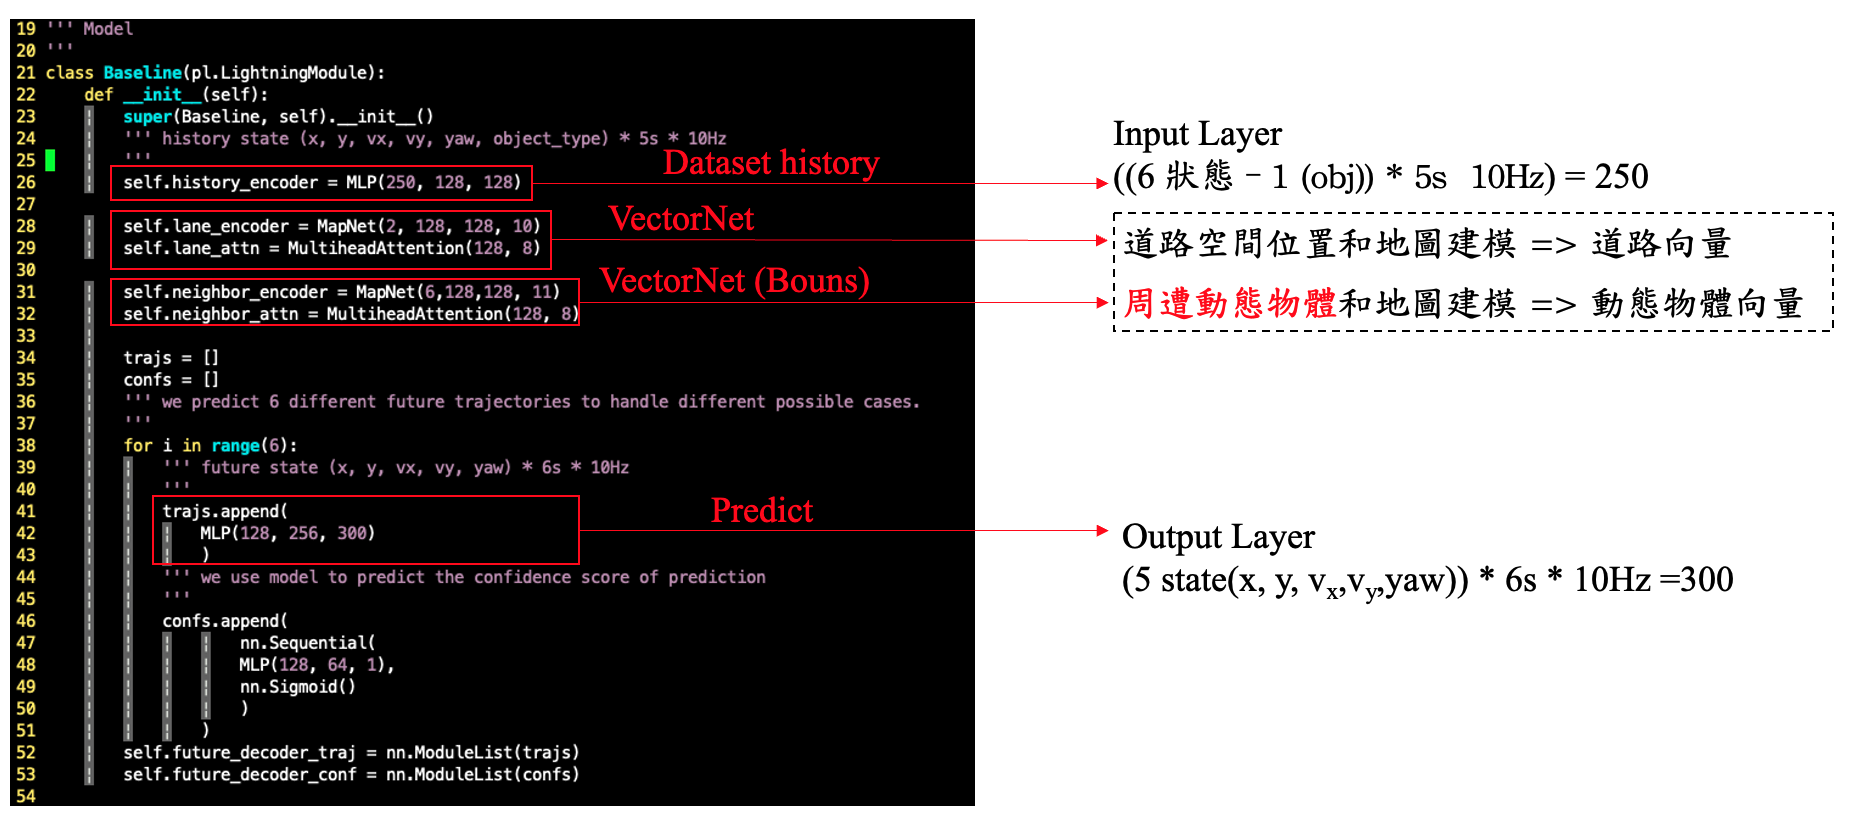
\includegraphics[scale=0.3]{./model1.png}
\end{figure}

\begin{figure}[H]
	\centering
	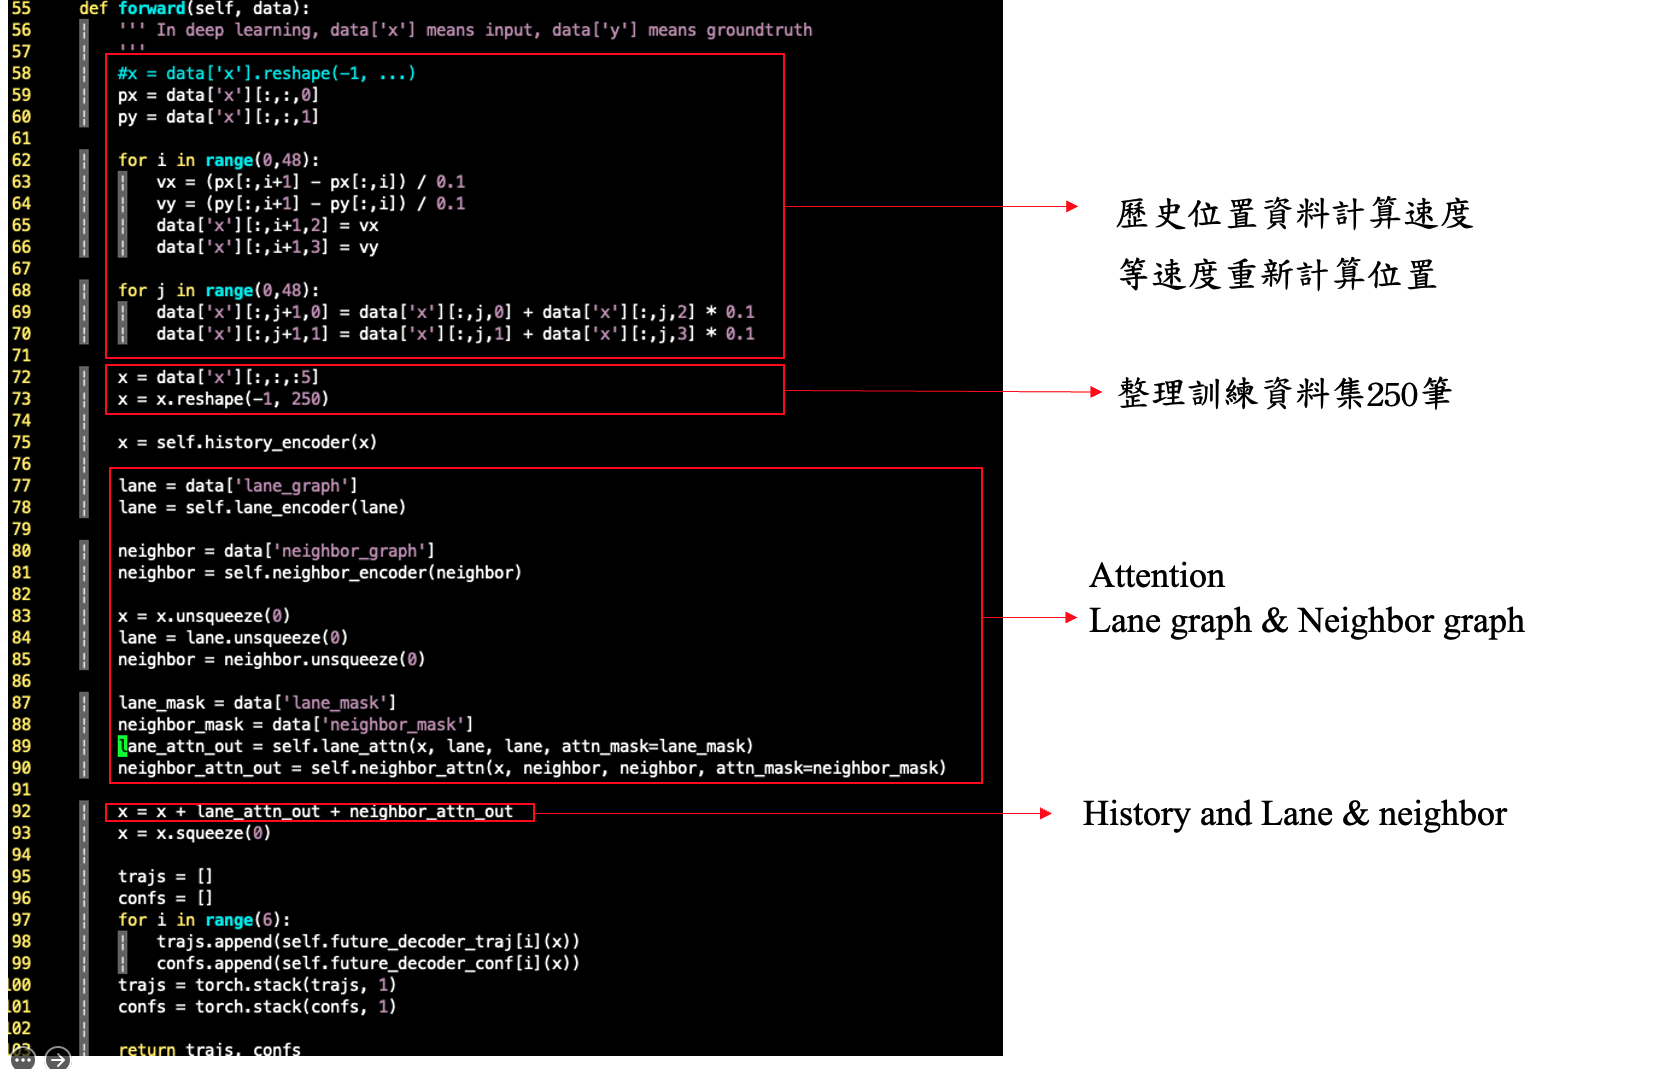
\includegraphics[scale=0.3]{./model2.png}
\end{figure}

\subsection{Case study}
Argo Dataset:以兩種方法調整解決路徑預測不佳問題
\begin{itemize}
	\item 可增加Epoch次數可降低train loss 而在ADE(Average Displacement Error) 及 FDE(Final Displacement Error)也可逐步降低。
	\item 而在加 Neighbor 的動態軌跡時有提高訓練收斂速度,可在較少Epoch達到最好的路徑。

\subsubsection{直線預測}
可成功預測出直線路徑,但Epoch100預測出直線有波浪現象因此多增加訓練次數效果較佳
\begin{figure}[H]
	\centering
	\subfigure[epoch 100]{
		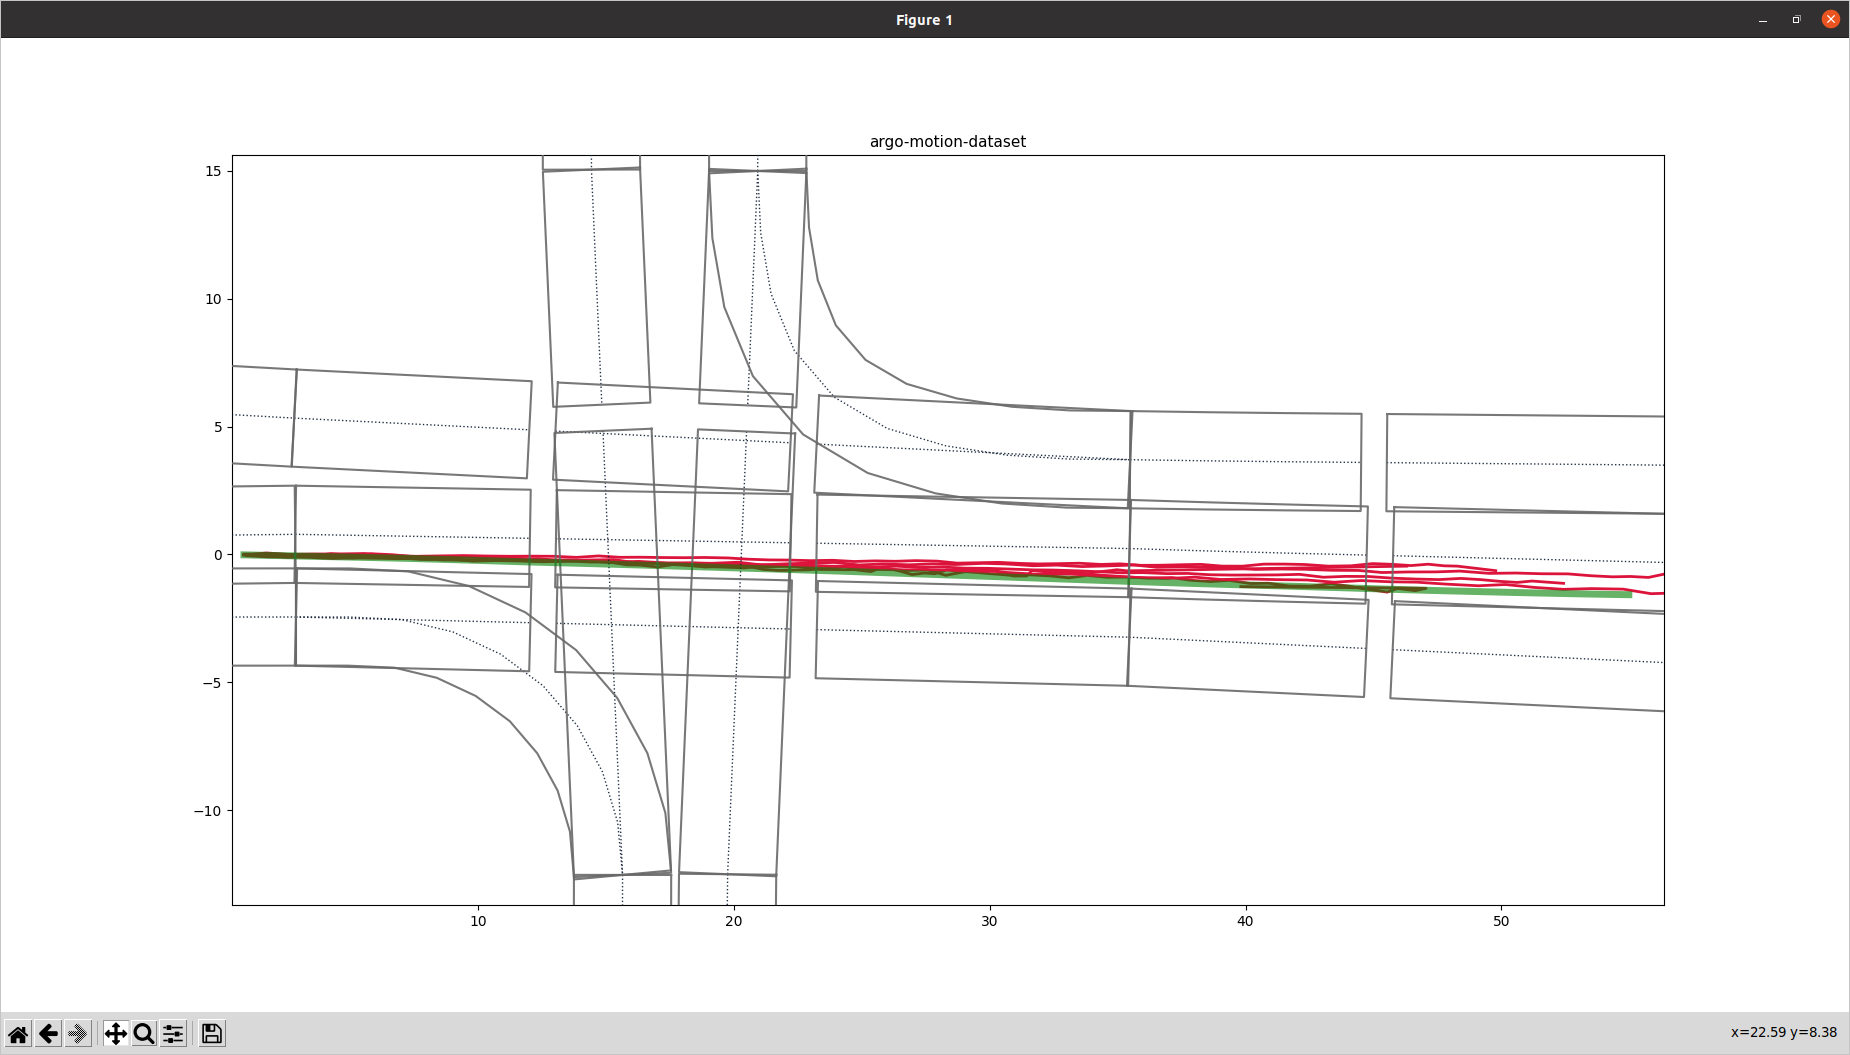
\includegraphics[width=0.4\textwidth]{./straight_100.png}
	}
	\subfigure[epoch 1000]{
		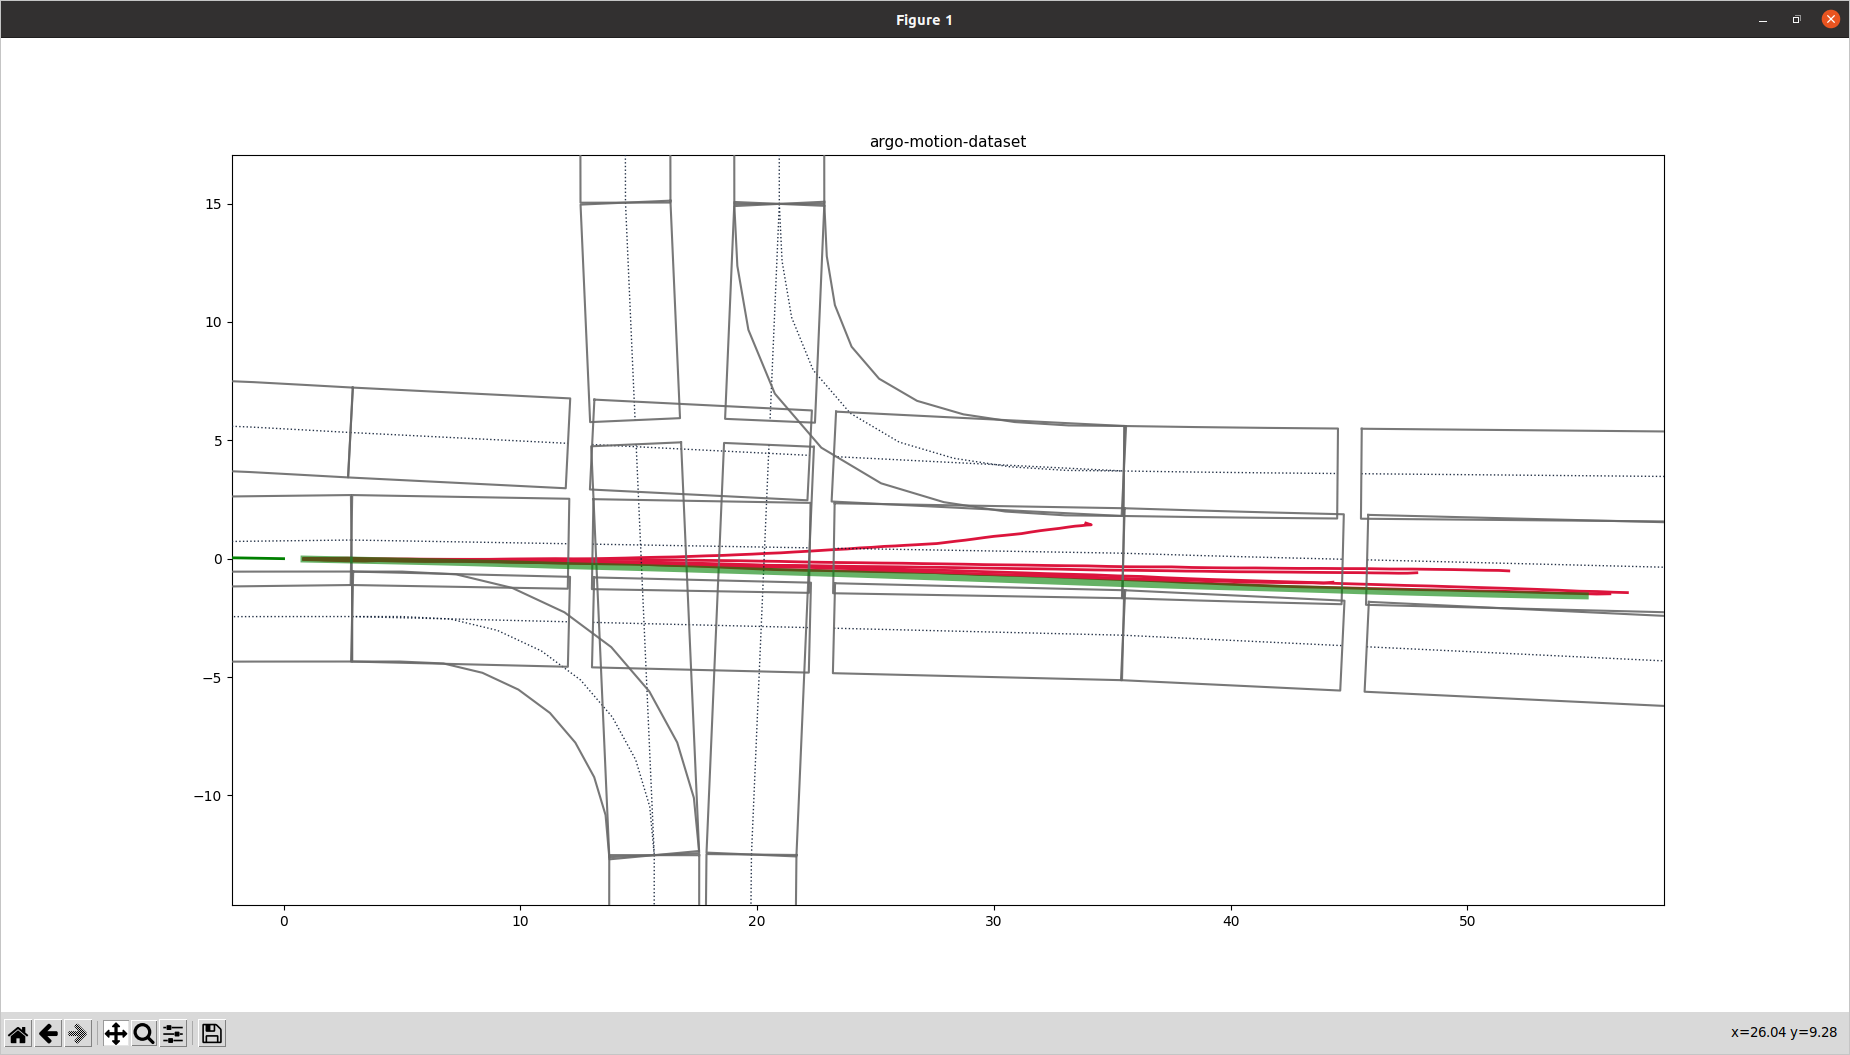
\includegraphics[width=0.4\textwidth]{./straight_1000.png}
	}
\end{figure}

\subsubsection{變換車道}
100Epoch無法正確預測變換車道結果,但經由增加Epoch可成功預測出結果。
\begin{figure}[H]
	\centering
	\subfigure[epoch 100]{
		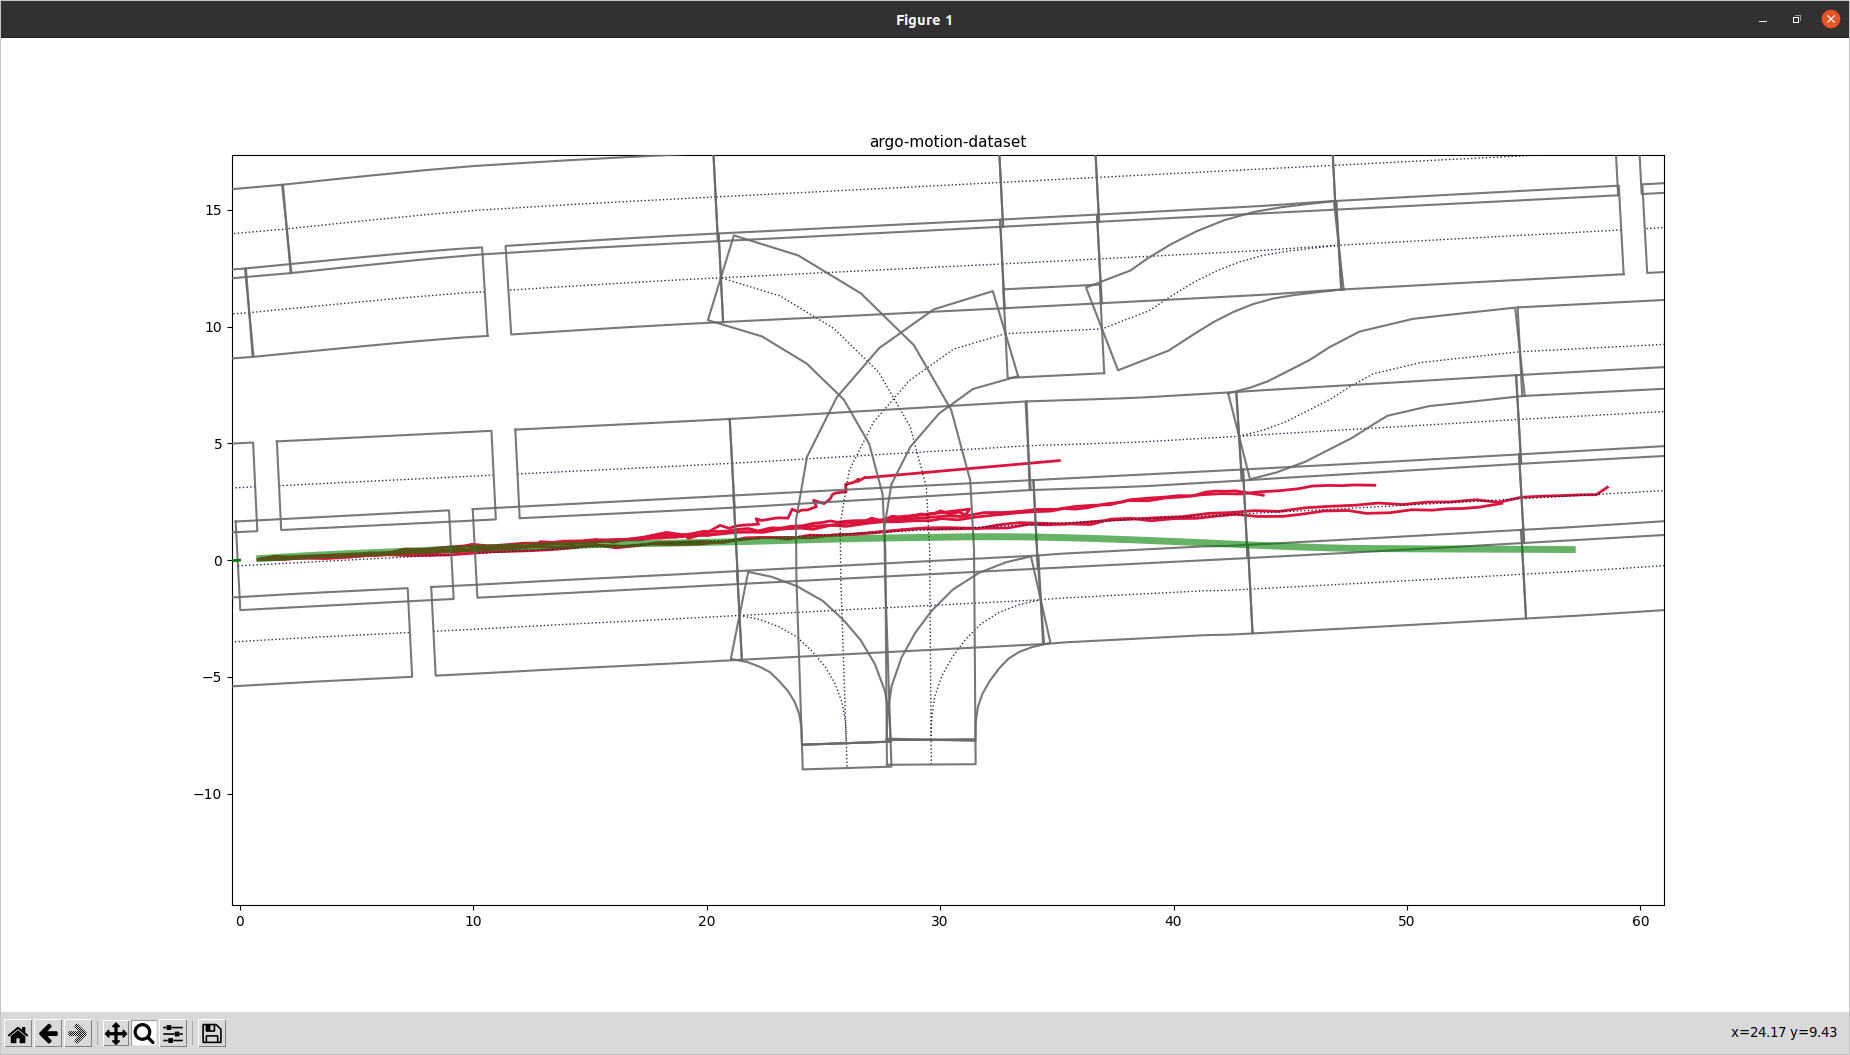
\includegraphics[width=0.4\textwidth]{./change_100.png}
	}
	\subfigure[epoch 1000]{
		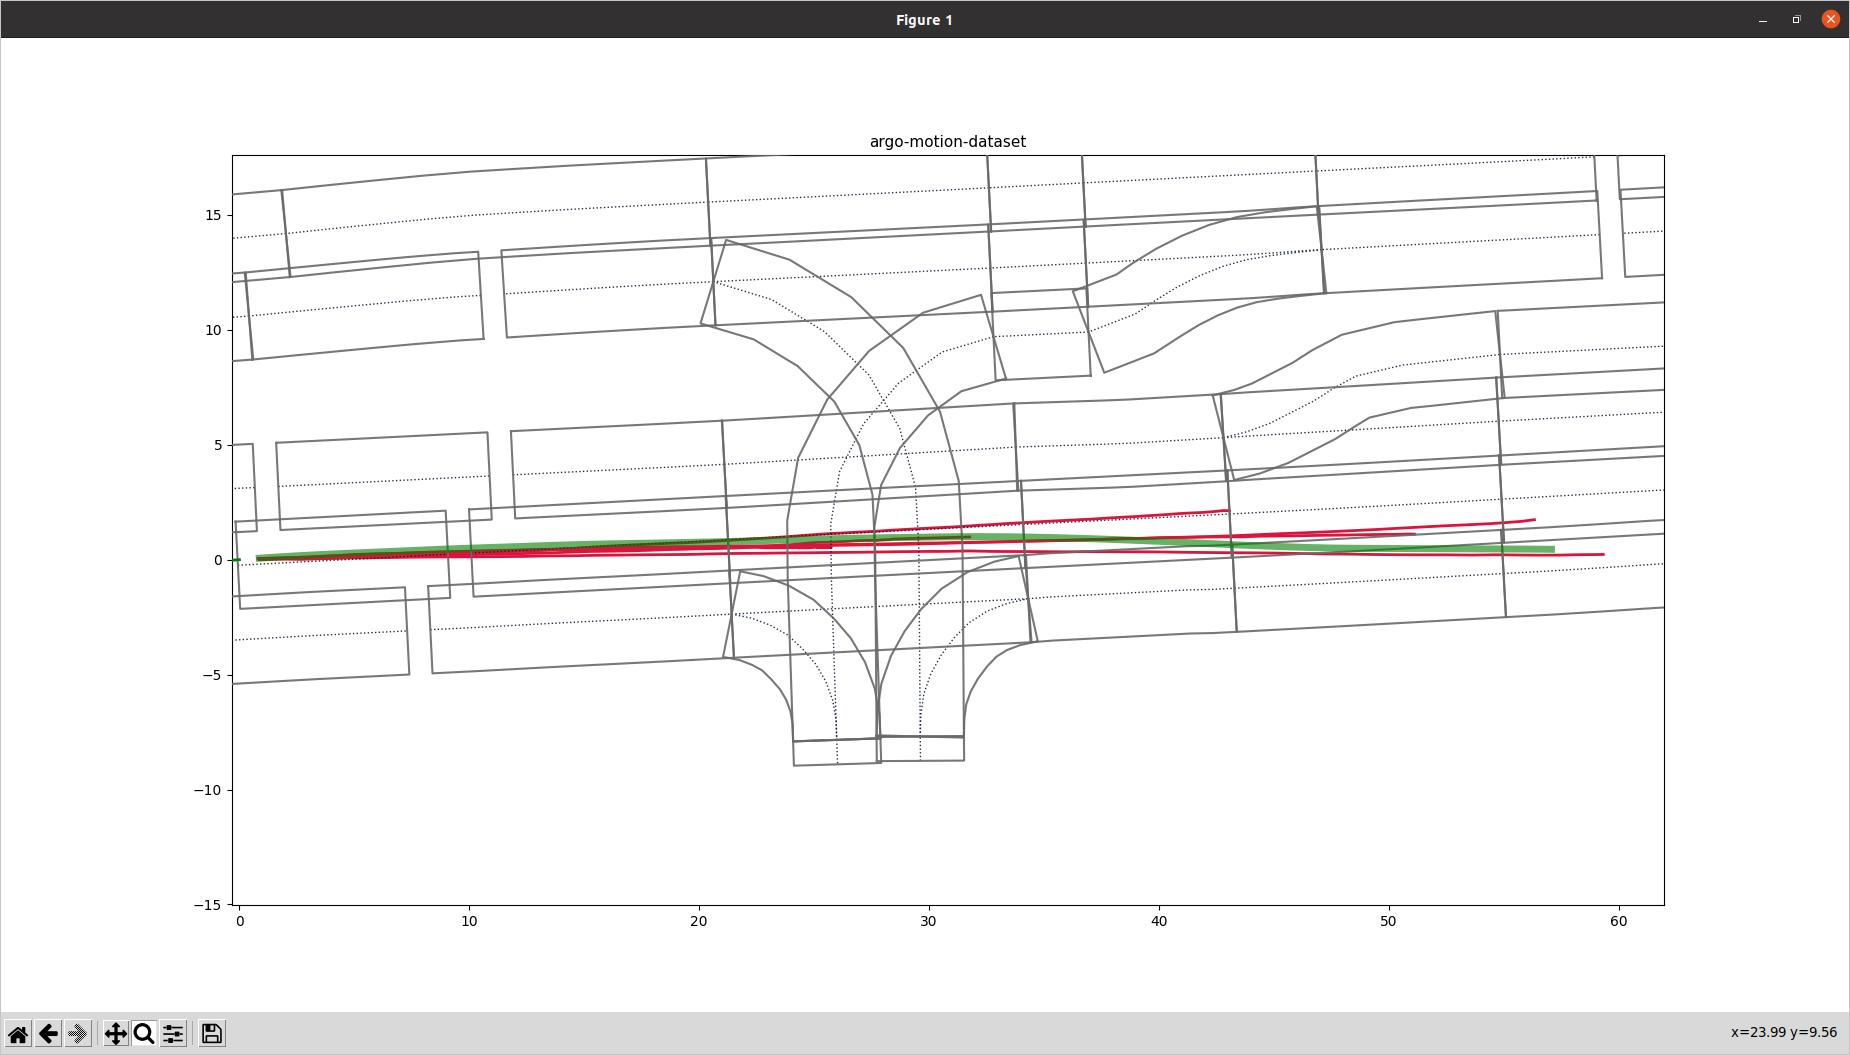
\includegraphics[width=0.4\textwidth]{./change_1000.png}
	}
\end{figure}

\subsubsection{車輛轉彎預測}
在100epoch及1000epoch都能預測出轉彎路徑,但1000epoch效果較好
\begin{figure}[H]
	\centering
	\subfigure[epoch 100]{
		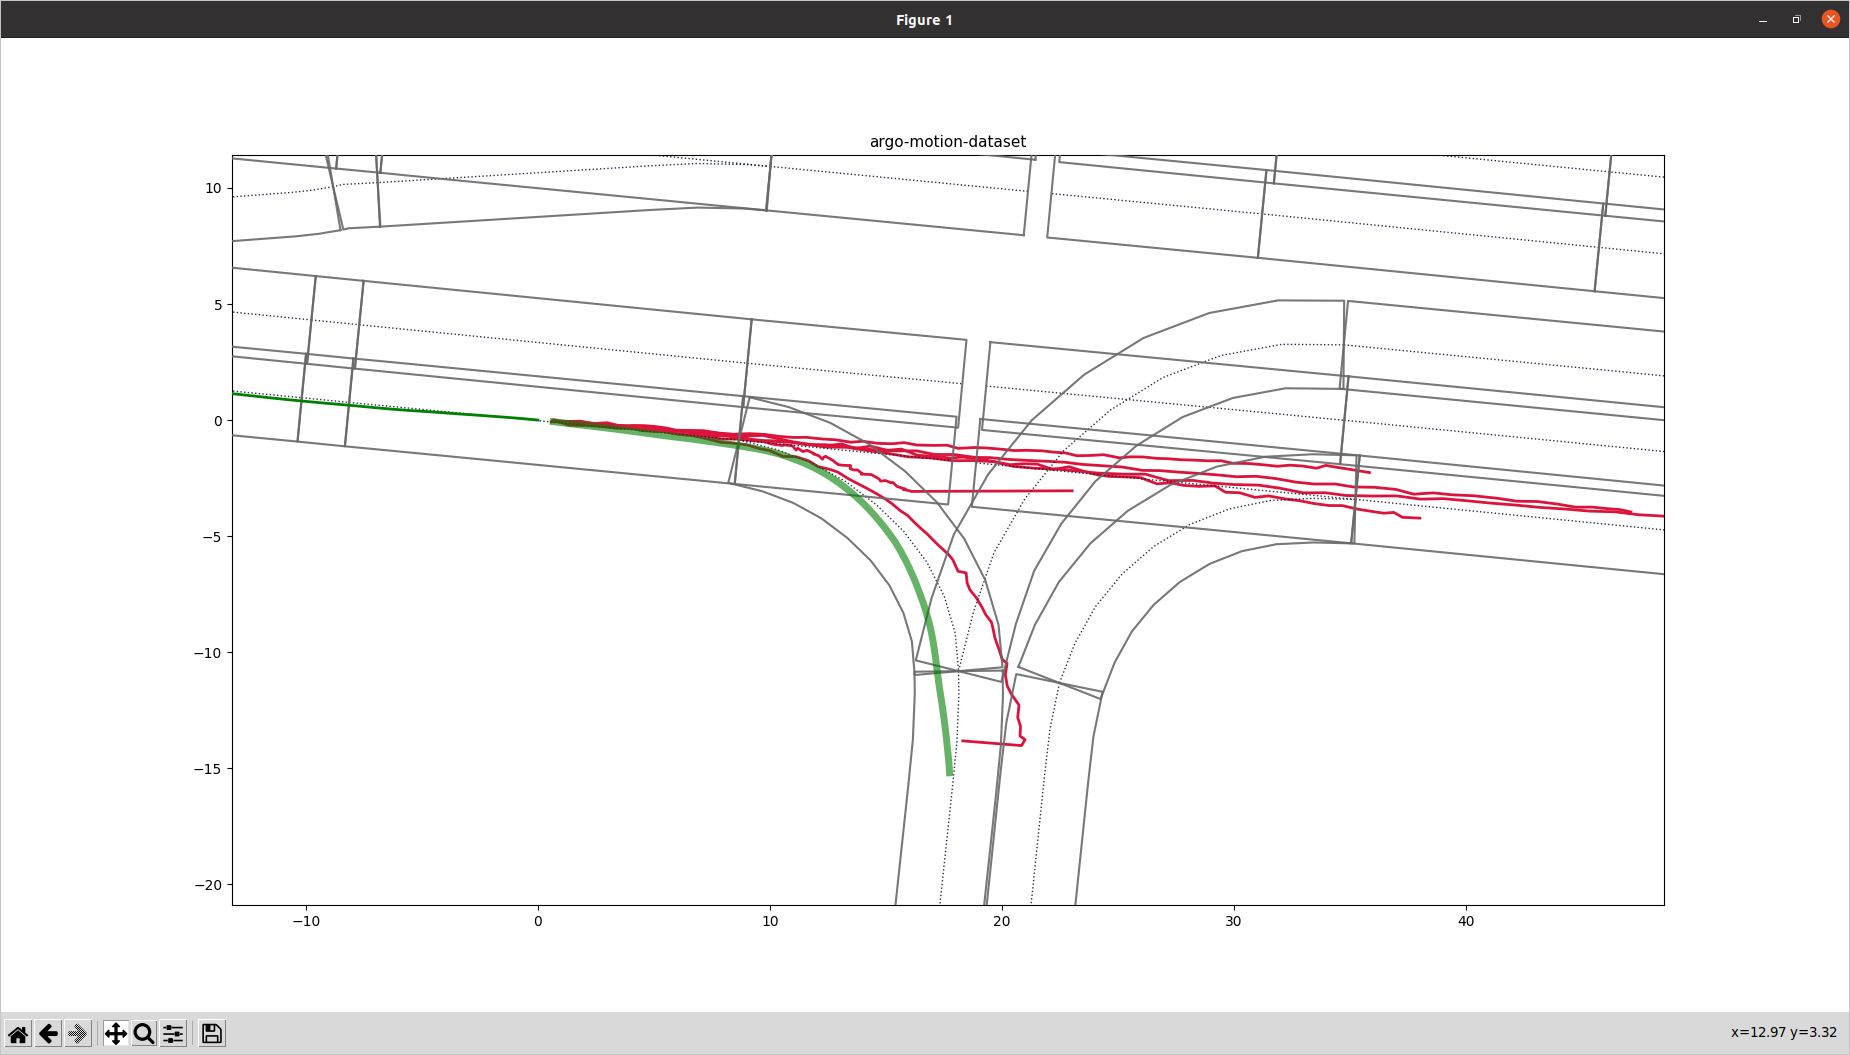
\includegraphics[width=0.4\textwidth]{./turn_100.png}
	}
	\subfigure[epoch 1000]{
		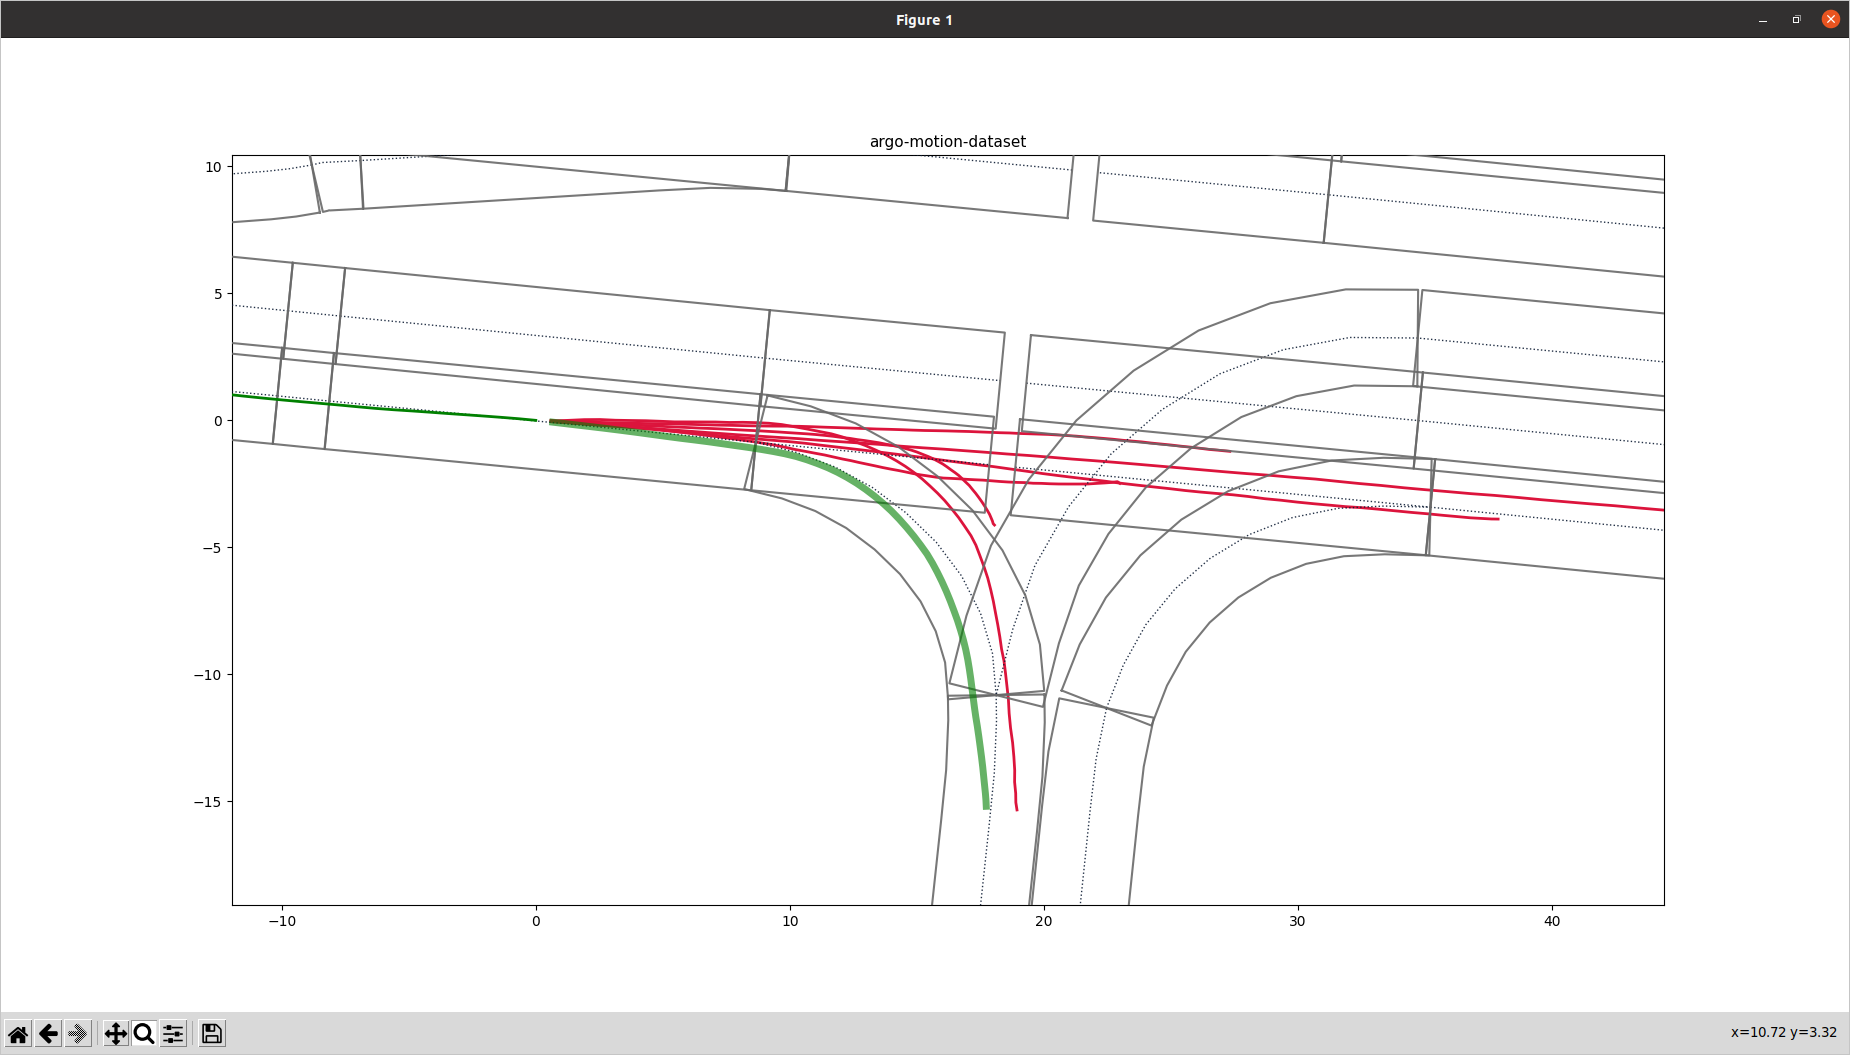
\includegraphics[width=0.4\textwidth]{./turn_1000.png}
	}
\end{figure}

\subsubsection{停止短路徑預測}
由於歷史資料少或是停止所造成路徑預測效果不佳,提高Epoch能增加預測結果。
\begin{figure}[H]
	\centering
	\subfigure[epoch 100]{
		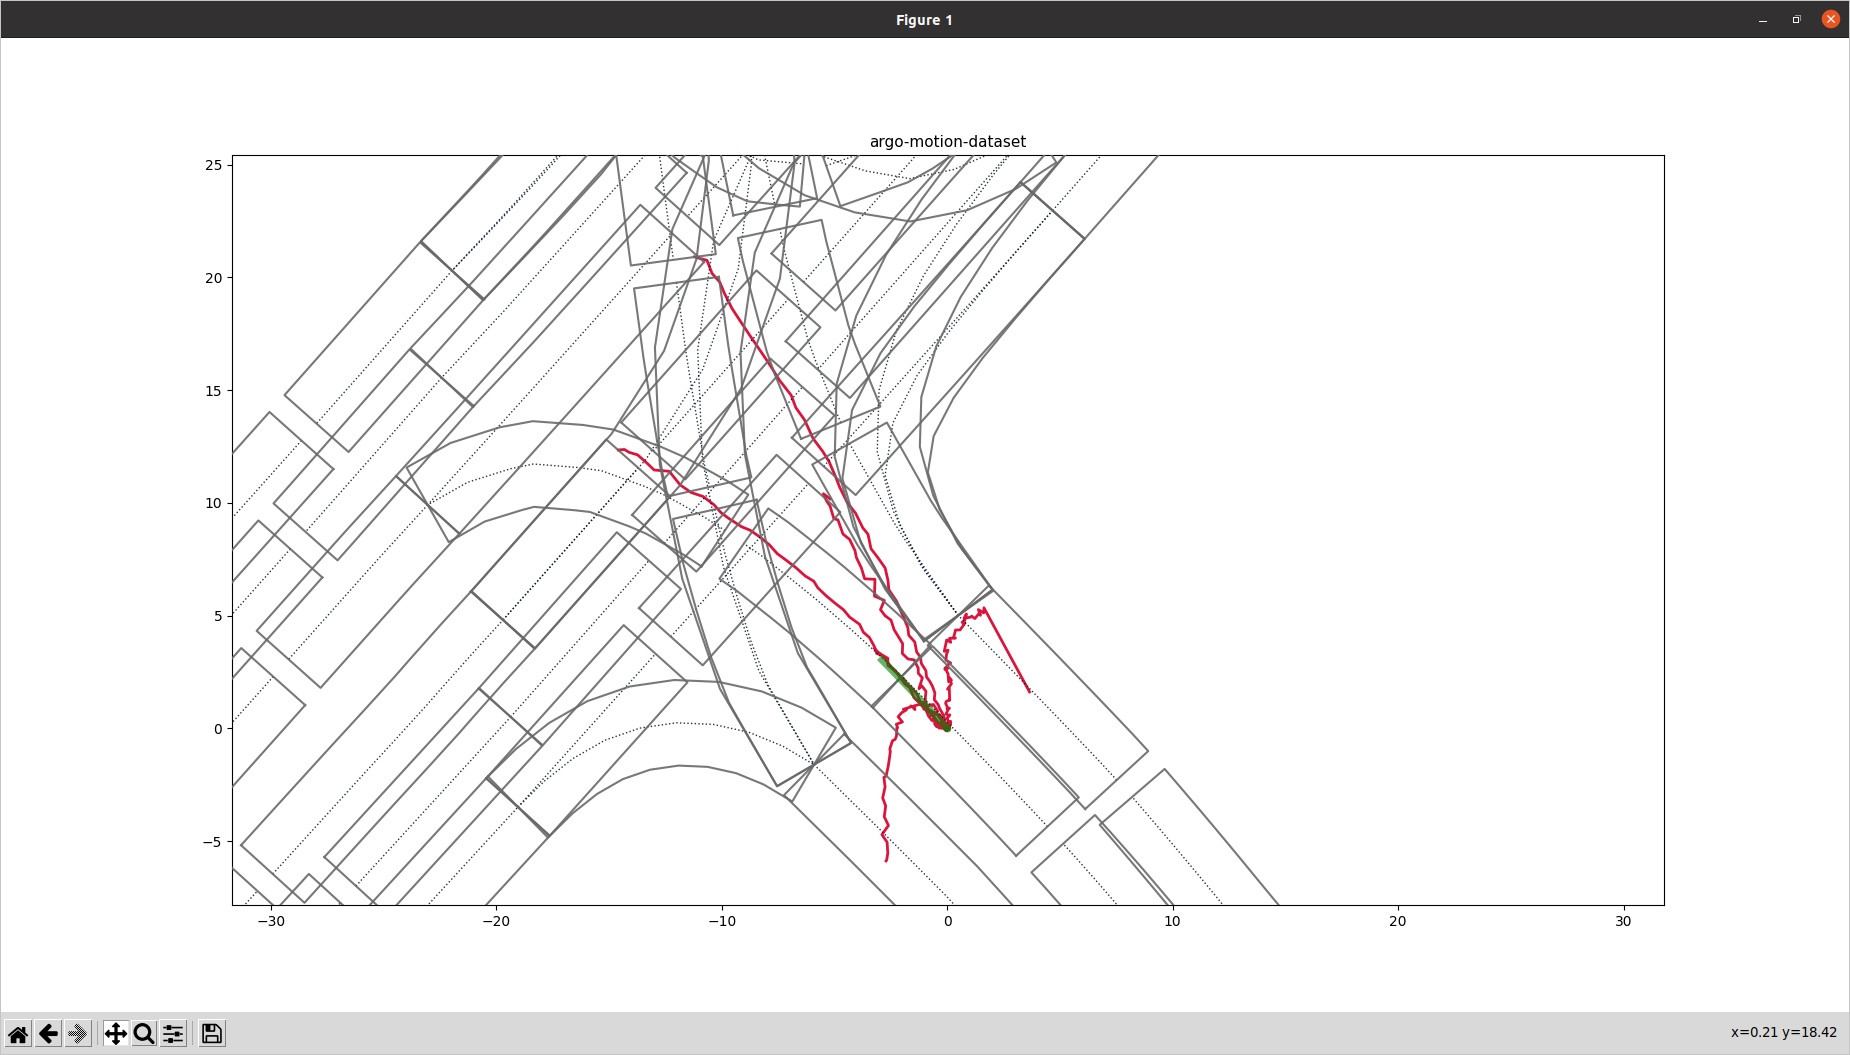
\includegraphics[width=0.4\textwidth]{./stop_100.png}
	}
	\subfigure[epoch 1000]{
		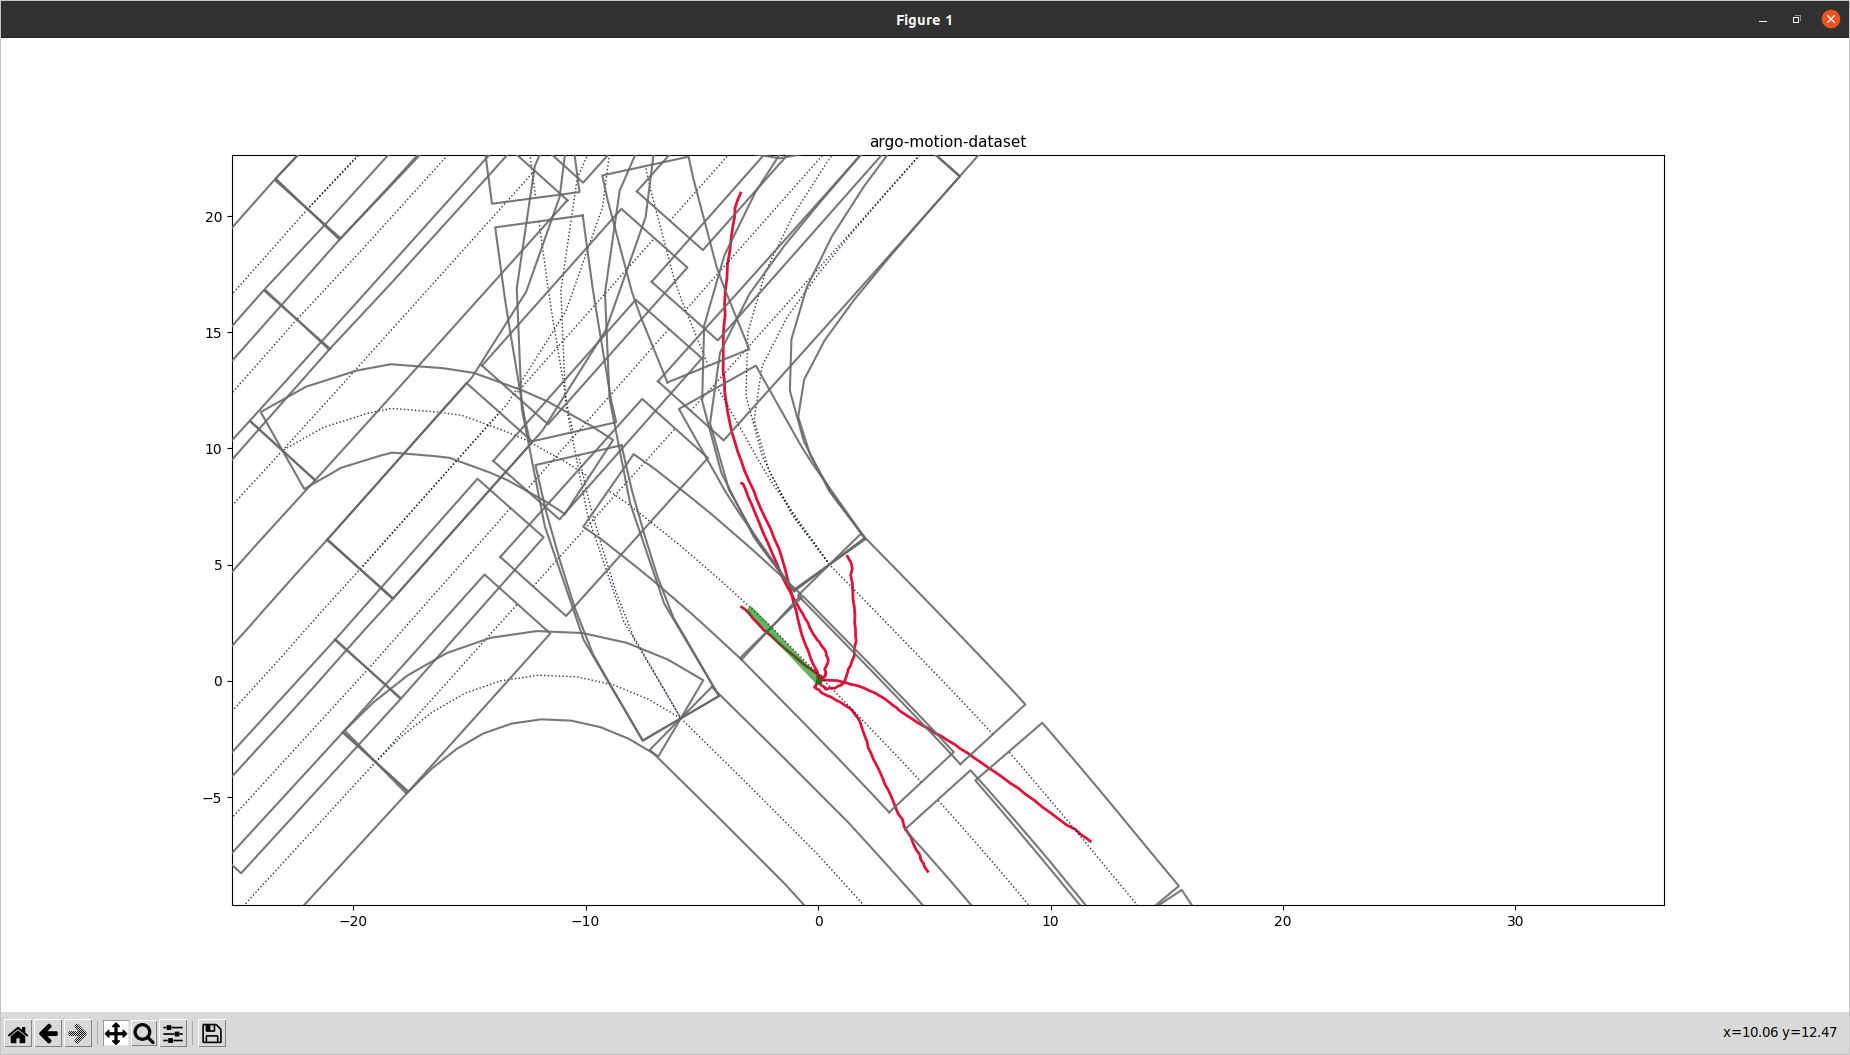
\includegraphics[width=0.4\textwidth]{./stop_1000.png}
	}
\end{figure}

\section{Kung Fu}

經由Argo訓練好的模型套用到光復路資料集做測試,經過實驗測試結果顯示同樣的模型套用的效果跟Argo Dataset相比略有差距,對於直線預測可以正常預測,但變換車道可能預測並不是相當好,而在轉彎處及停止可正確預測出。

\subsection{變換車道}
Epoch100無法預測出變換車道,而在1000 epoch 已預測出切換車道但不完整可能需要在增加Epoch效果應該能更好
\begin{figure}[H]
	\centering
	\subfigure[epoch 100]{
		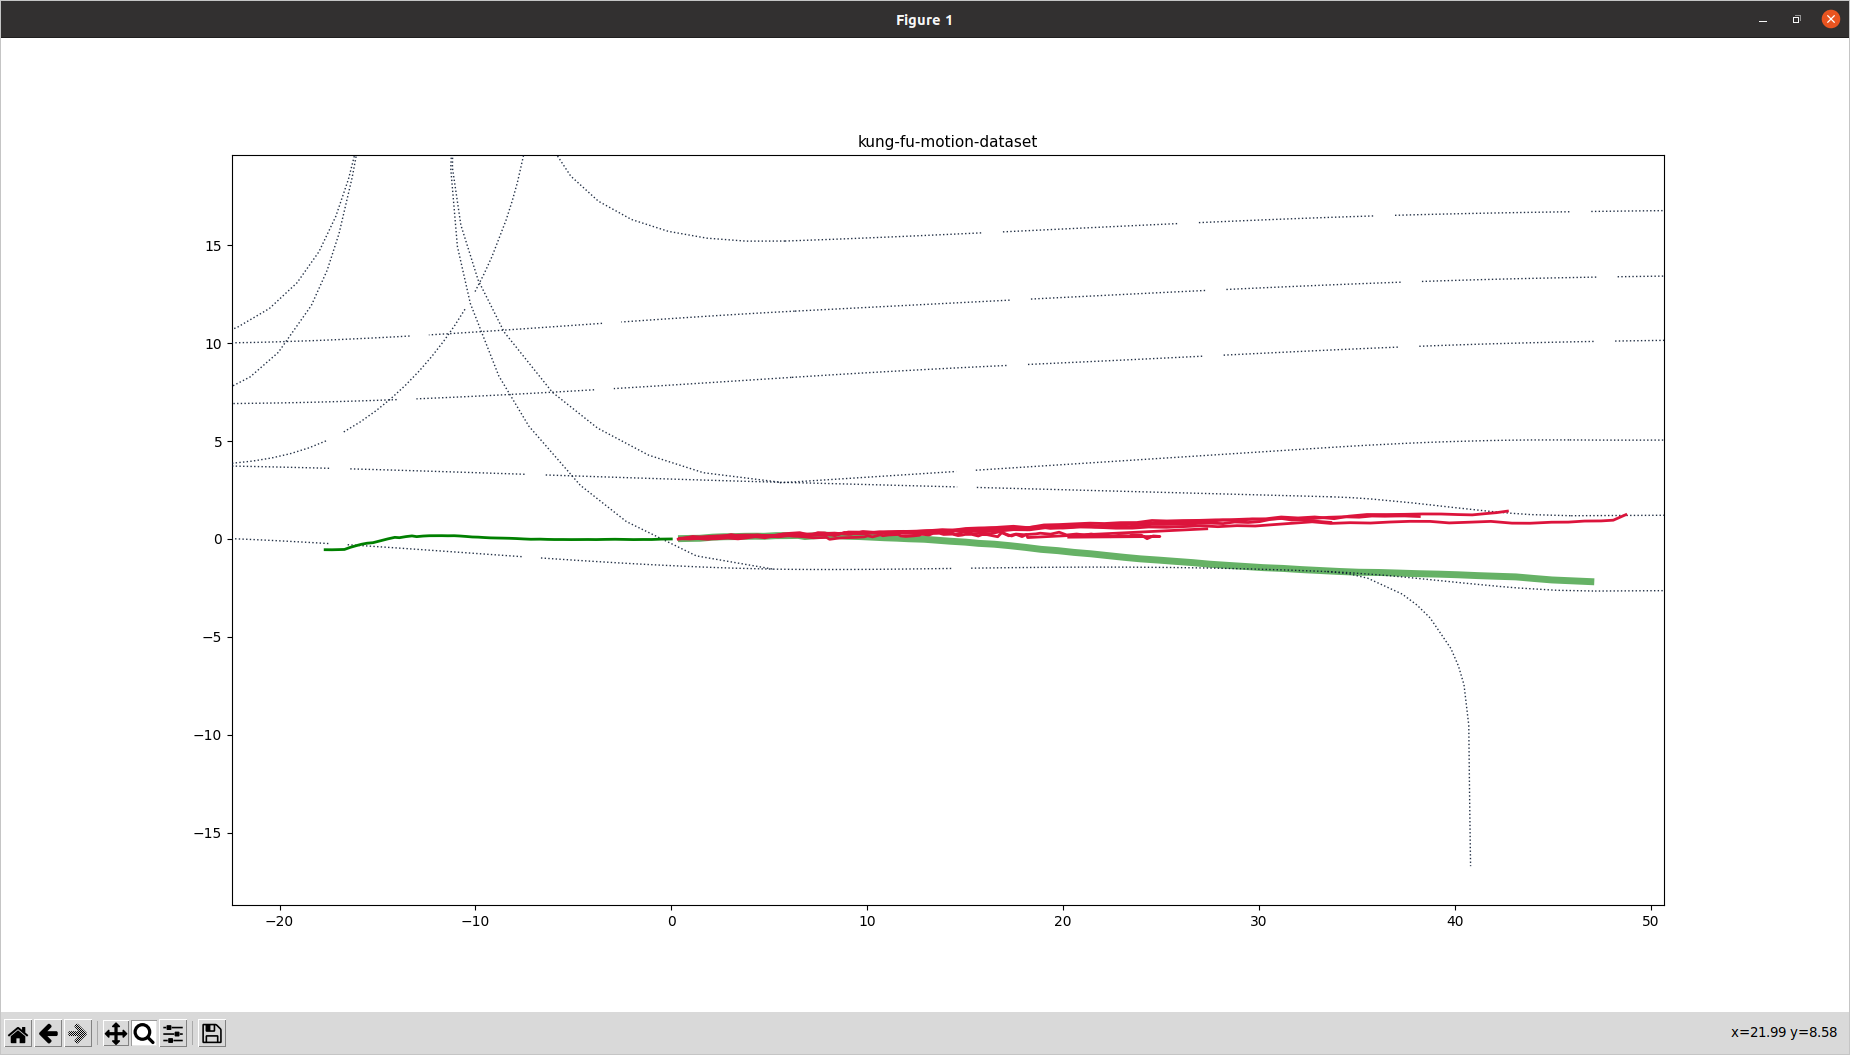
\includegraphics[width=0.4\textwidth]{./kungfu100/kungfu_s100.png}
	}
	\subfigure[epoch 1000]{
		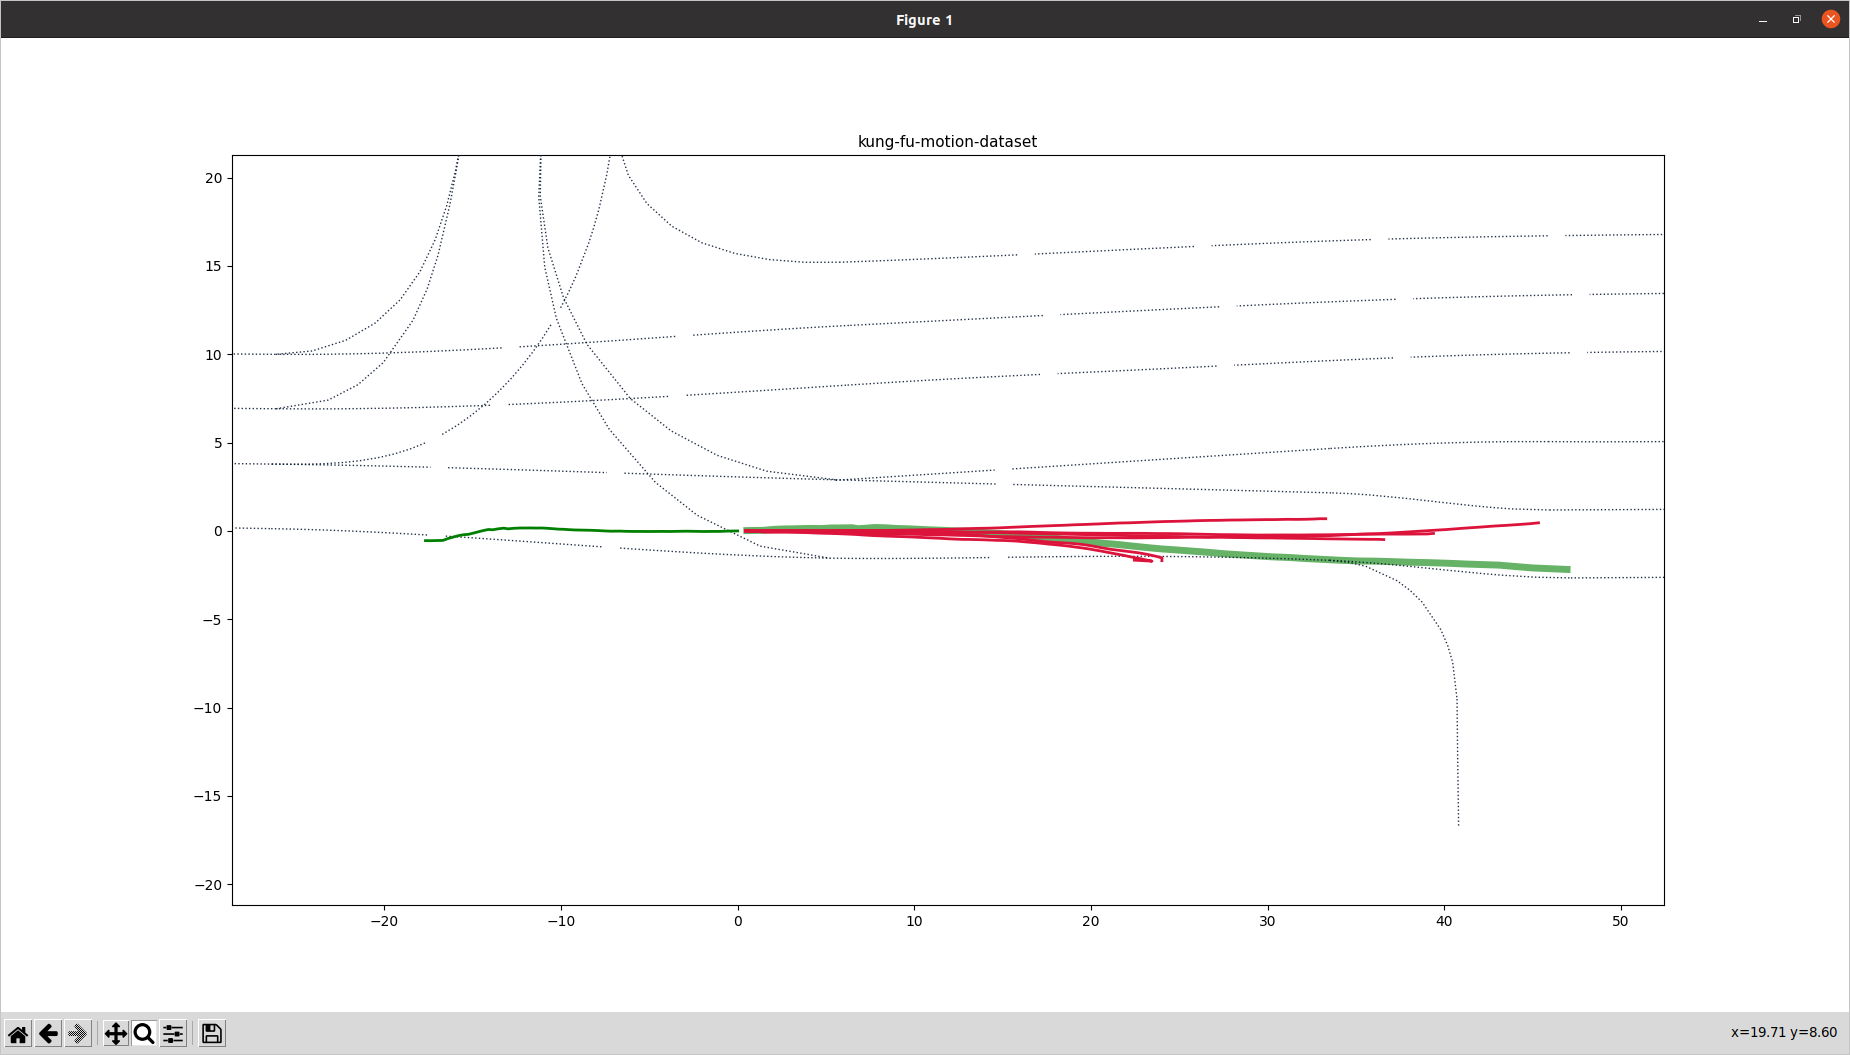
\includegraphics[width=0.4\textwidth]{./kungfu1000/kungfu_s1000.png}
	}
\end{figure}

\subsection{車輛轉彎}
相比之下100 epoch 卻比起1000 epoch預測的更好,可得到並非訓練多次效果會越好。
\begin{figure}[H]
	\centering
	\subfigure[epoch 100]{
		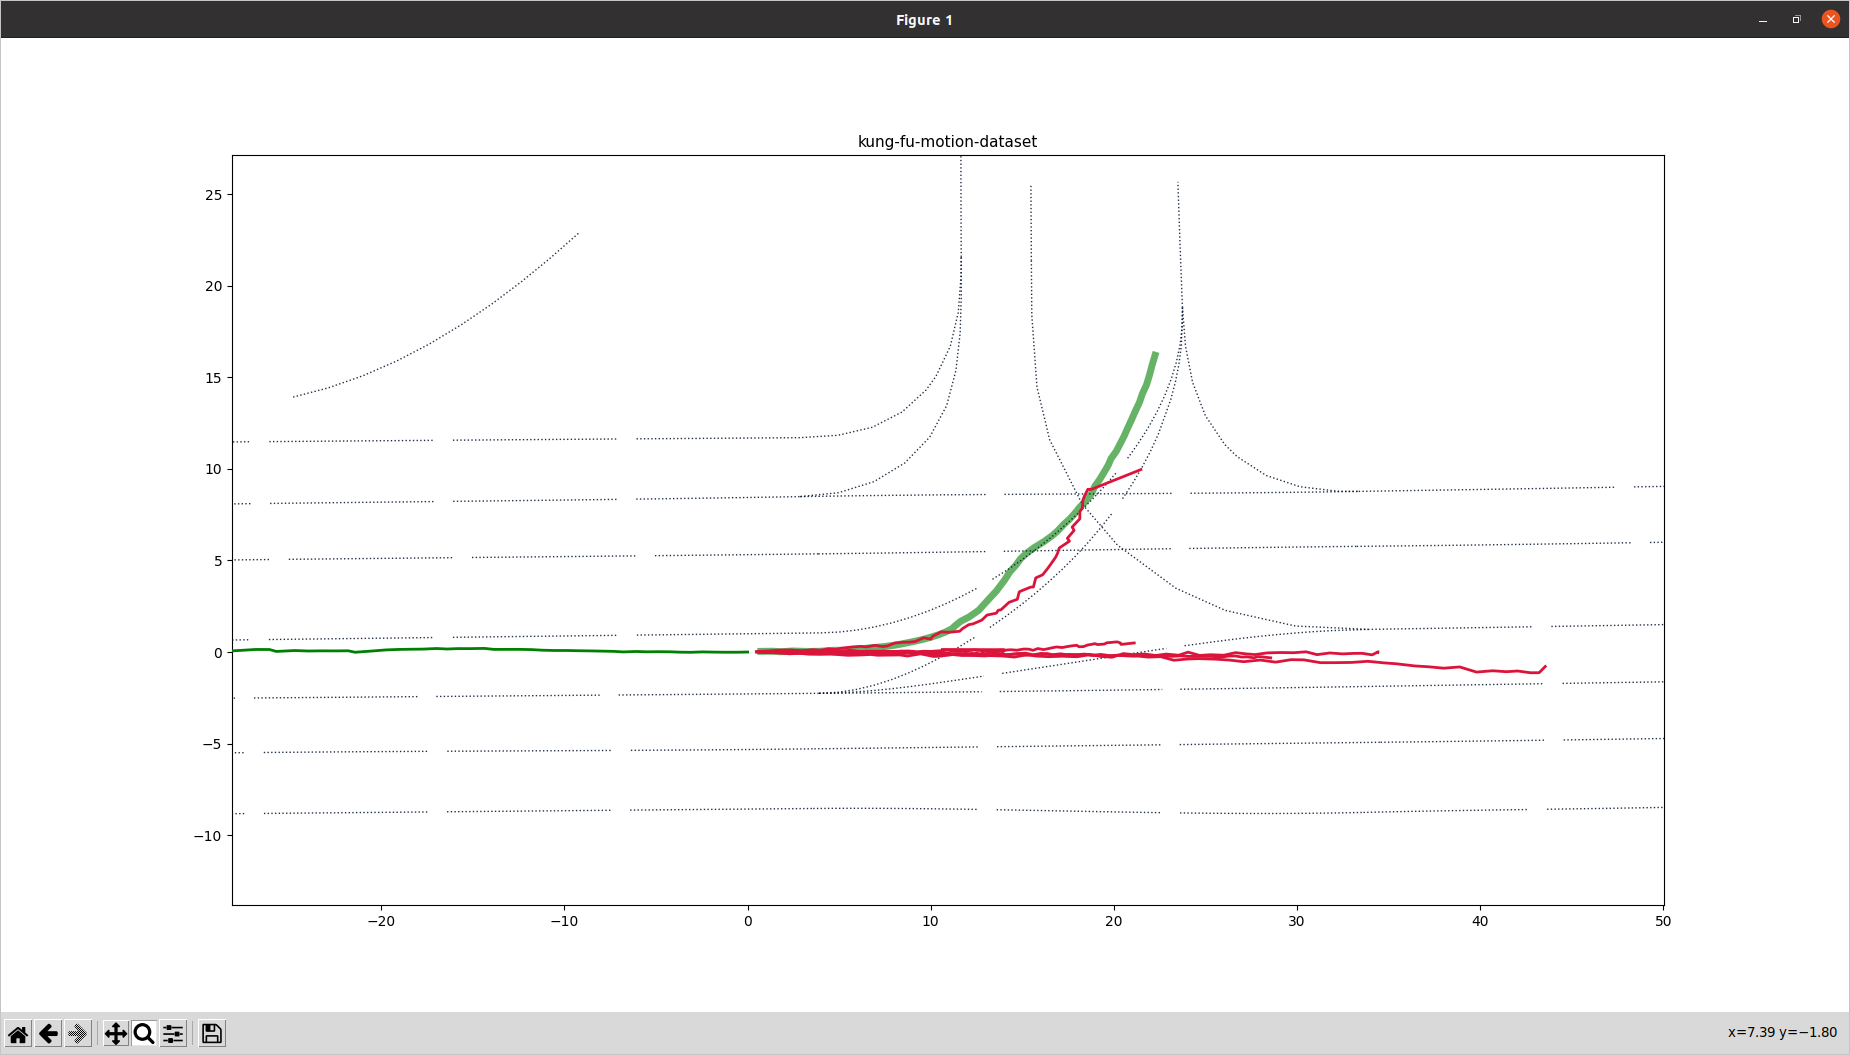
\includegraphics[width=0.4\textwidth]{./kungfu100/kungfu_t100.png}
	}
	\subfigure[epoch 1000]{
		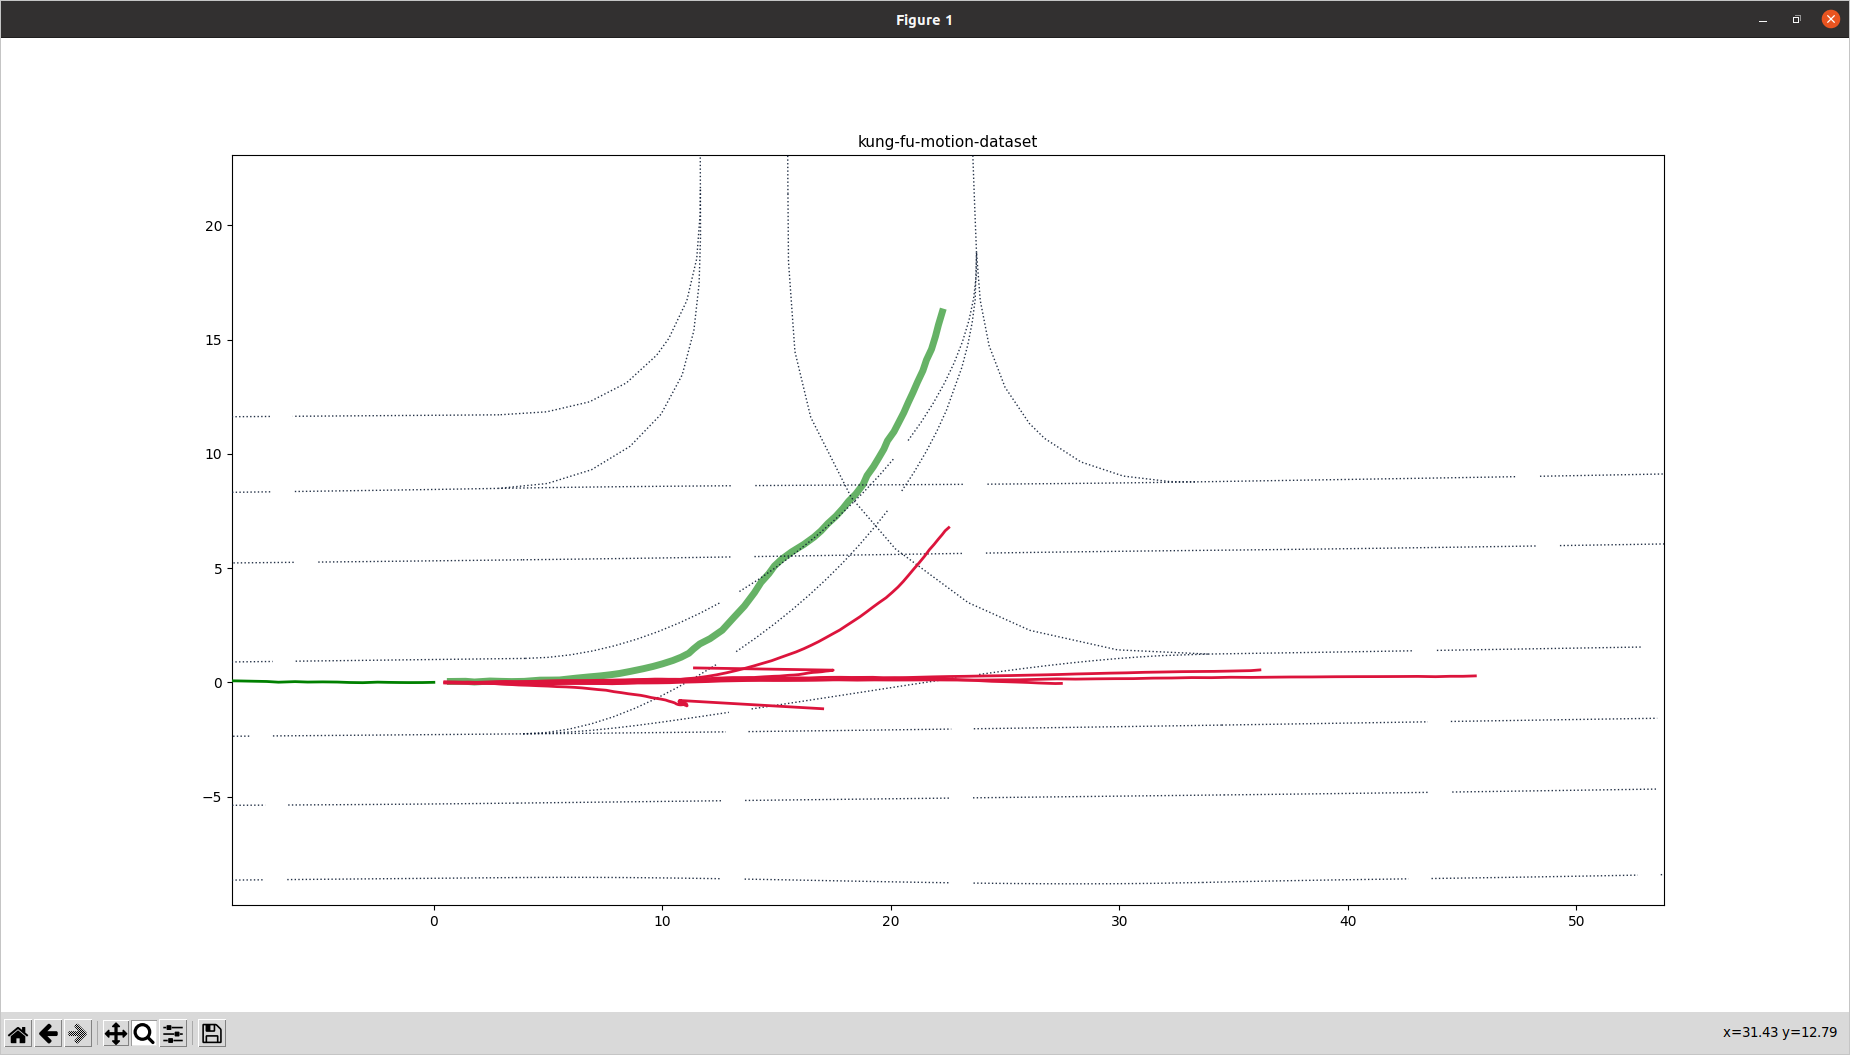
\includegraphics[width=0.4\textwidth]{./kungfu1000/kungfu_t1000.png}
	}
\end{figure}

\subsection{車輛停止}
車輛停止在1000 epoch 有成功預測出,但100epoch未能預測出車輛停止
\begin{figure}[H]
	\centering
	\subfigure[epoch 100]{
		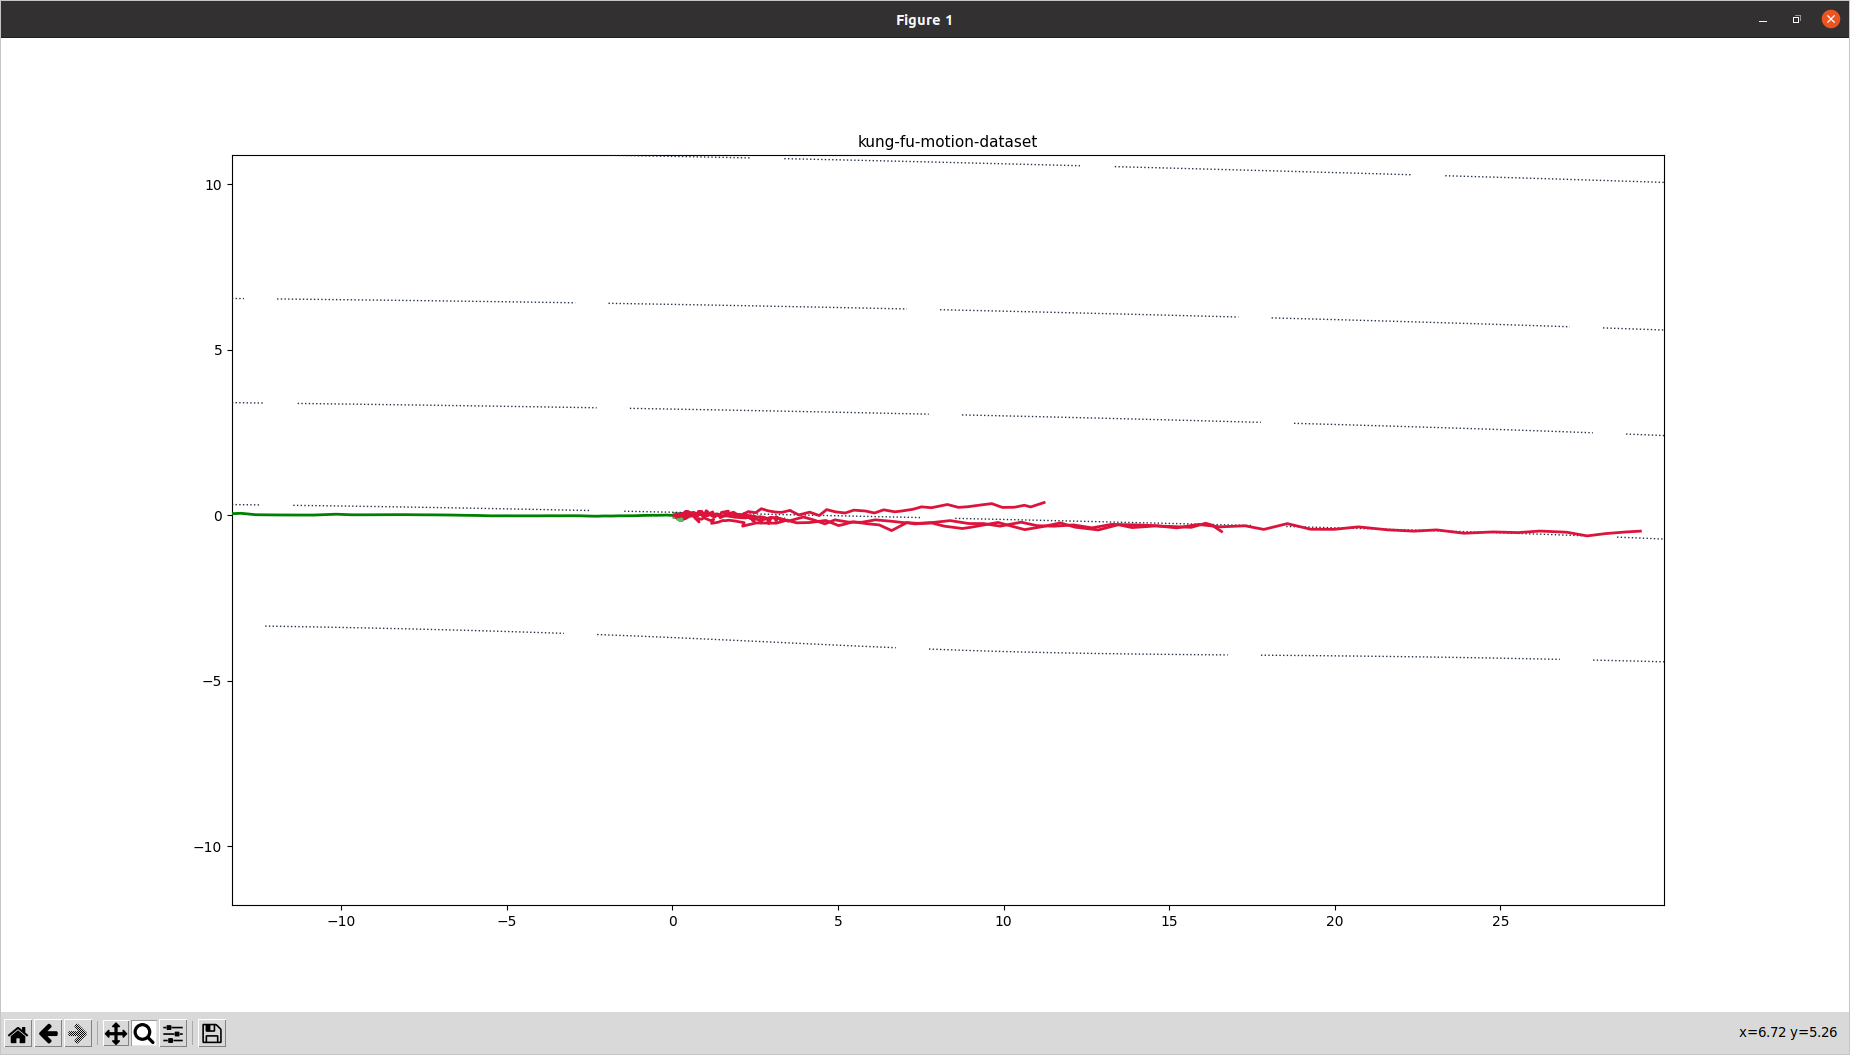
\includegraphics[width=0.4\textwidth]{./kungfu100/kungfu_stop100.png}
	}
	\subfigure[epoch 1000]{
		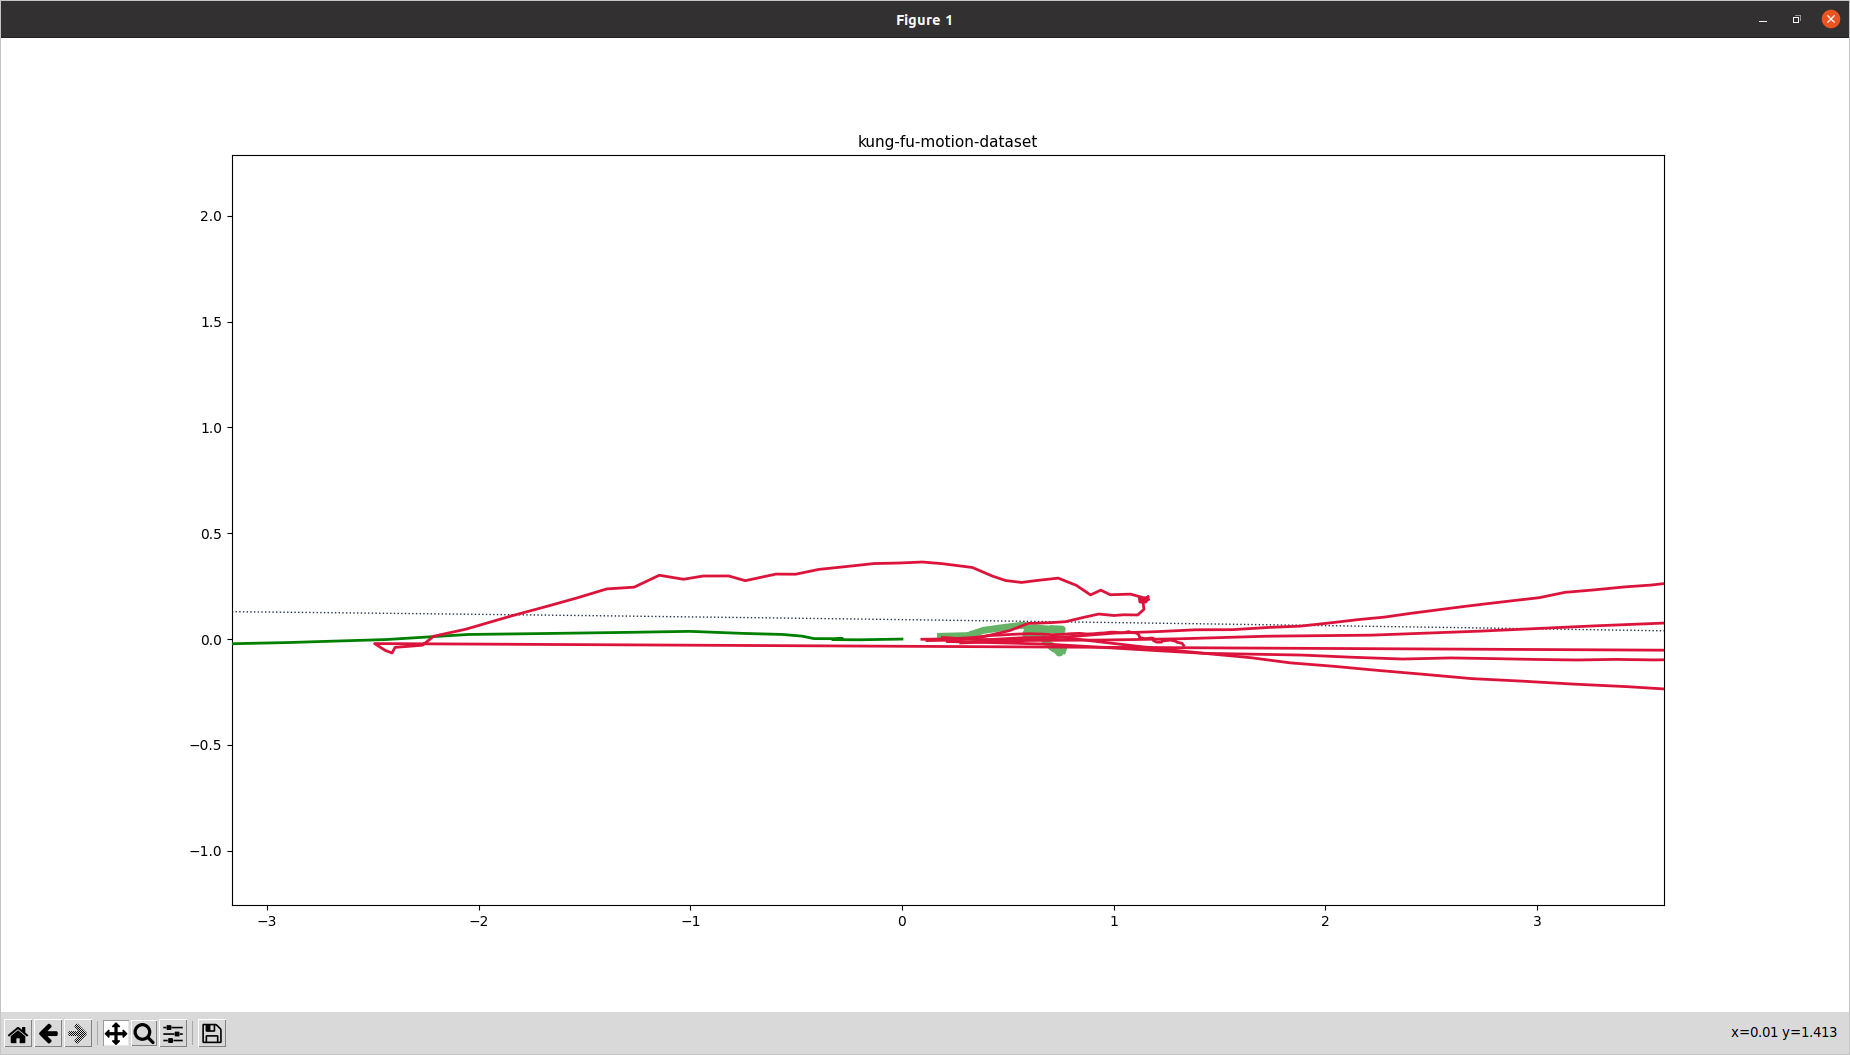
\includegraphics[width=0.4\textwidth]{./kungfu1000/kungfu_stop1000.png}
	}
\end{figure}



\begin{thebibliography}{1}

\bibitem{1}
	Liang, M., Yang, B., Hu, R., Chen, Y., Liao, R., Feng, S., Urtasun, R. (2020, August). Learning lane graph representations for motion forecasting. In European Conference on Computer Vision (pp. 541-556). Springer, Cham.
\bibitem{2}
	Gao, J., Sun, C., Zhao, H., Shen, Y., Anguelov, D., Li, C., Schmid, C. (2020). Vectornet: Encoding hd maps and agent dynamics from vectorized representation. In Proceedings of the IEEE/CVF Conference on Computer Vision and Pattern Recognition (pp. 11525-11533).
\end{thebibliography}


\end{document}
